\documentclass[10pt,twocolumn,letterpaper]{article}

\usepackage{eso-pic}
\usepackage{cvpr}
\usepackage{times}
\usepackage{epsfig}
\usepackage{graphicx}
\usepackage{amsmath}
\usepackage{amssymb}
\usepackage{xspace}
\usepackage{booktabs}


% Include other packages here, before hyperref.
\usepackage{my_macros}
\usepackage{paralist}
\usepackage{amsthm}
\usepackage{dirtytalk}
%\usepackage{framed}
\usepackage{caption}
\usepackage{subcaption}
\usepackage{algorithm}
%\usepackage{algorithmic}
\usepackage{algpseudocode}
\usepackage{setspace}
%for tikz
\usepackage{tikz,pgfplots}
\usepackage{pgfplotstable}
\usepackage{filecontents}
\usetikzlibrary{arrows,positioning,automata,shadows,fit,shapes}
\usetikzlibrary{arrows,petri,topaths}
\usetikzlibrary{positioning,fit,calc}
\usetikzlibrary{shapes.arrows,chains,decorations.pathreplacing,fadings}
\usetikzlibrary{calc, matrix, backgrounds}

\pgfplotsset{every axis/.append style={
  every axis y label/.style = {at={(ticklabel cs:0.5)}, rotate=90, anchor=south},
  axis x line = {bottom},
  axis y line = {left},
  tick align = outside,
  ymajorgrids = true,
%  legend style = {draw=none, at={(1.05, 0.5)}, anchor=west, font=\small},
  legend style = {font=\tiny},
  legend columns = 1,
  every axis plot/.append style = {line width=1pt},
  label style = {font=\small},
  tick label style={font=\small},
  scaled ticks = false,
}}

\usepackage{tkz-berge}
\DeclareMathOperator*{\argmin}{arg\,min}
\DeclareMathOperator*{\argmax}{arg\,max}
\definecolor{shadecolor}{rgb}{0.01,0.199,0.1}
\usepackage{xargs} 
\newtheorem{theorem}{Theorem}

% If you comment hyperref and then uncomment it, you should delete
% egpaper.aux before re-running latex.  (Or just hit 'q' on the first latex
% run, let it finish, and you should be clear).
\usepackage[pagebackref=true,breaklinks=true,letterpaper=true,colorlinks,bookmarks=false]{hyperref}

\def\arraystretch{0.8}
\renewcommand{\tabcolsep}{2pt}
\newcommand{\thickline}{2pt}
\newcommand{\scatterplotpath}{./scatterplots/}

\usepackage[colorinlistoftodos,prependcaption,textsize=tiny]{todonotes}
\newcommandx{\unsure}[2][1=]{\todo[linecolor=red,backgroundcolor=red!25,bordercolor=red,#1]{#2}}
\newcommandx{\change}[2][1=]{\todo[linecolor=blue,backgroundcolor=blue!25,bordercolor=blue,#1]{#2}}
\newcommandx{\info}[2][1=]{\todo[linecolor=OliveGreen,backgroundcolor=OliveGreen!25,bordercolor=OliveGreen,#1]{#2}}
\newcommandx{\improvement}[2][1=]{\todo[linecolor=Plum,backgroundcolor=Plum!25,bordercolor=Plum,#1]{#2}}
\newcommandx{\thiswillnotshow}[2][1=]{\todo[disable,#1]{#2}}


% \cvprfinalcopy % *** Uncomment this line for the final submission

\def\cvprPaperID{****} % *** Enter the CVPR Paper ID here
\def\httilde{\mbox{\tt\raisebox{-.5ex}{\symbol{126}}}}

% Pages are numbered in submission mode, and unnumbered in camera-ready
\ifcvprfinal\pagestyle{empty}\fi
\begin{document}
%%%%%%%%% TITLE
%!TEX root = egpaper_for_review.tex
\newcommand{\Cut }{\mathcal{C}}
%\title{Correlation Clustering with Dynamic Super-Nodes (DySNCC)}
\title{Fusion Moves for Correlation Clustering}

\author{First Author\\
Institution1\\
Institution1 address\\
{\tt\small firstauthor@i1.org}
% For a paper whose authors are all at the same institution,
% omit the following lines up until the closing ``}''.
% Additional authors and addresses can be added with ``\and'',
% just like the second author.
% To save space, use either the email address or home page, not both
\and
Second Author\\
Institution2\\
First line of institution2 address\\
{\tt\small secondauthor@i2.org}
}

\maketitle
%\thispagestyle{empty}


\listoftodos[Notes]
%%%%%%%%% ABSTRACT
\begin{abstract}
   We address the problem of partitioning a  graph
   into a previously unknown number of clusters.
   Among all partitions, the one with the minimal 
   sum of of cut edge weights is chosen. 
   This problem is known as correlation clustering 
   or multicut.
   We propose a general framework to find
   high quality approximate solutions for 
   this NP-hard problem based on a move making algorithm:
   We use candidate solutions from a proposal generator
   to iteratively improve the best observed solution similar
   to fusion moves.
   The proposed solver outperforms any other solver
   w.r.t. to any time performance.
   The solutions found by this solver are close
   to global optimal solutions w.r.t. energy
   and problem specific measurements as VI for
   image segmentation problems.

\end{abstract}
\section{Introduction}

\begin{itemize}
  \item Multicut in computer vision, applications, sparse segmentation -> IMPORTANT PROBLEM
  \item Problem: Existing Methods does not scale, even CGC. - Large scale 3d problems
  \item Contribution: Fast scalable method using novel fusion moves for correlation clustering
\end{itemize}



\todo[inline]{should there be a general introduction to multicuts?}


Given an edge weighted graph, positive weights (\emph{attractive})
encourage the adjacent nodes to be in the same 
connected component, while negative weights (\emph{repulsive}) encourage
the nodes to stay in different connect components.
Therefore the sign of the weights encodes if two
nodes should be merged or not and the magnitude of the weights encodes
the certainty of this desire.
The objective of correlation clustering / multicuts
is finding the cut with a minimal sum of cut edge weights.
The number of connected components / clusters is discovered
from the weights ( rewrite?!?).
Correlation clustering / the multicut is NP-hard \cite{???}.
%
Despite the NP-hardness, correlation clustering has been 
successfully used for
\begin{inparaenum}[(i)]
    \item partitioning a superpixel region adjacency graph~\cite{andres_2011_iccv,kroeger_2012_eccv}
    \item with optional long range repulsive edges~\cite{andres_2013_emmcvpr}.
    \item Alush and Globerger showed how to average multiple segmentations with the multicut objective~\cite{alush_2012_pami}.
    \item Multicuts can also be used for interactive segmentation~\cite{bagon_2011_arxiv},
    \item for co-segmentation~\cite{glassner_2011_cvpr}
    \item and to cluster fully connected graphs~\cite{???}.
\end{inparaenum}





\todo[inline]{WHY WE NEED THIS NEW SOLVER?}


Nunez-Iglesias \etal describe the multicut as
\say{one-shot agglomeration of supervoxels} whose 
main drawback is the scalability \cite{nunez_iglesias_2013}.

\todo[inline]{BETTER MOTIVATE SUPERNODES}

To address scalability, supernodes can be useful.
To create supernodes, some edges will be contracted
and their nodes are merged into super-nodes.
Doing so, we can reduce  the graph 
to a reasonable size, such that we can find
global optimal multicut solutions within reasonable time.
%
Any edge which is contracted is lost.
If such an edge is cut in the global optimal solution, we cannot 
find this global optimal solutions.
Therefore we avoid fixed decisions and use a
dynamic energy aware contraction scheme.
%
Different edge contractions lead to different super-node graphs.
A trivial approach is the following.
Create different super-node graphs, optimize them with multicuts,
and take the result which leads to the lowest energy
on the unmodified initial graph.
% 
Doing so, we throw away all results which do not have the lowest energy.
Within this work we propose a framework which 
combine multiple \emph{proposal} super-node graphs
without any premature irreversible decisions.
Furthermore, multiple super-node graphs are combined such
that the information form all of them is used.
\todo[inline]{\emph{proposal} super-node graphs sounds shitty}
%
The proposed algorithm can be interpreted as a fusion moves
algorithm for correlation clustering / multicut objective.
We generate cheap and versatile proposals
and \emph{fuse} them with the current best solution with the
guarantee that this cannot increase the energy.


\textbf{Contribution:}

\textbf{Outline:}

%-------------------------------------------------------------------------

\section{Problem Formulation}
Def: Graph, weighted graph, cut, multicut 


\begin{center}
    \begin{eqnarray}
        l^* &=& \argmin_{L \in \{1,\ldots,|V|\}^{|V|}} \sum_{ (i,j) \in E } w_{ij} \cdot [l_{u} \neq l_{v}] \label{eq:nodeproblem}\\
   %     y_{ij}^* &=& [l_{u} \neq l_{v}] 
        y^* &=& \argmin_{y \in MC(G)\cap \{0,1\}^{|E|}} \sum_{ (i,j) \in E } w_{ij} \cdot y_{ij} \label{eq:edgeproblem}%\\ 
    \end{eqnarray}
\end{center}

The exist an surjective mapping from a node-label $l$ to edge-labeling $y$ and
a bijective mapping from a partitioning of $V$ to vertices of the multicut polytope $MC$.
Consequently, 
(i) problems \ref{eq:nodeproblem} and \ref{eq:edgeproblem} are equivalent
and (ii) the node-labeling is not unique for a given partitioning and introduce some
ambiguities.

% \subsubsection{Multicut Objective}

% The multicut / correlation clustering objective 
% can be formulated in different ways.



% \paragraph{Edge Indicator Variables:}
% \begin{center}
%     \begin{eqnarray}
%         y^* &=& \argmin_{y} \sum_{ e_{ij} \in E } w_{ij} \cdot y_{ij} \\
%         s.t.:& & y \in \textit{Multicut Polytope} \nonumber
%     \end{eqnarray}
% \end{center}

% \paragraph{Fully Connected Graph:}
% \begin{center}
%     \begin{eqnarray}
%         y^*   & = & \argmin_{y} \sum_{ i<j \in V } w_{ij} \cdot y_{ij} \\
%         s.t.: &  & y_{ij} + y_{jk} < y_{i,k} \quad \forall i, j, k   \nonumber
%     \end{eqnarray}
% \end{center}

% \paragraph{Node Coloring:}
% \begin{center}
%     \begin{eqnarray}
%         l^* &=& \argmin_{L} \sum_{ e_{ij} \in E } w_{ij} \cdot [l_{u} \neq l_{v}] \\
%         y_{ij}^* &=& [l_{u} \neq l_{v}]  
%     \end{eqnarray}
% \end{center}

\section{Related Work}

% \subsubsection{Solver for the Multicut Objective}
    
    %!TEX root = ../egpaper_for_review.tex
\begin{table}
\begin{center}
    \begin{tiny}
    \begin{tabular}{ p{1cm} p{1cm} p{1.5cm} p{2.5cm} }
    \hline
    \hline
    Method &    & Limitations &   \\ \hline
    Multicut \cite{andres_2011_iccv,kappes_2011_emmcvpr} & 
        (I)LP & 
        not scalable, slow &
        Cutting plane method.
        Global optimal but slow for huge problems. 
        However, applicable for medium size superpixel RAG. 
        \\ \hline
    Expand And Explorer \cite{bagon_2011_arxiv} & 
        movemaker & 
        gets stuck early &
        $\alpha$-Expansion modification. Applicable to
        large scale problems but gets stuck in local minima(???).
        \\ \hline
    Fast Planar CC \cite{yarkony_2012_eccv} & 
        dual-decompositon & 
        planar graphs only, 
        duality/integrality gab &
        Dual decompositon in planar subgraphs??
        Works on planar graphs only. Fast (is there a word for fast to medium fast) for
        small to medium size graphs.
        \\ \hline
    Cut Glue and Cut \cite{beier_2014_cvpr} & 
        move-making & 
        gets stuck in poor minima for non planar graphs &
        Greedy solver based on a series of 2 colorings.
        State of the art any time performance. Very
        fast for planar graphs. Gets stuck in local minima
        for non planar graphs.
        \\ \hline
    THIS WORK & 
        fusion move-making & 
        no natural stopping condition &
        Fusion of a proposal segmentation with
        the current best segmentation.
        State of the art any time performance for (???)
        \\ \hline
        \hline
    \end{tabular}
    \end{tiny}
\end{center}
\caption{
    Overview of correlation clustering / multicut solvers
}
\end{table}


\subsection{Correlation Clustering}
   \begin{itemize}
   \item Multicut~\cite{kappes_2011_emmcvpr}
   \item Expand and Explorer~\cite{bagon_2011_arxiv}
   \item Fast Planar CC~\cite{yarkony_2012_eccv}
   \item Break and Conquer \cite{alush_2013_simbad}.
   \item Cut Glue And Cut~\cite{beier_2014_cvpr}
   \end{itemize}

\subsection{Fusion Moves}
Move making algorithms, in particular fusion moves, 
have become increasingly popular for energy minimization~\cite{???,kappes_2014_ws}.
For many large scale computer vision applications fusion moves lead to good approximations
with state of the art any time performance~\cite{kappes_2014_ws}.




% \subsection{Karger-Stein Algorithms}
% Use randomized procedure to reduce the number of nodes / edges to a reasonable 
% number.
% On the smaller graph, more expensive solvers are used.



%------------------------------------------------------------------------
\section{Correlation-Clustering-Fusion (CCF) Moves}
Motivation Using Fusion moves -> problem ambiguity


%!TEX root = ../egpaper_for_review.tex
\begin{figure}[H]

\tikzfading[name=fade right0,left color=transparent!0, right color=transparent!70]
\tikzfading[name=fade right1,left color=transparent!70, right color=transparent!100]
\tikzstyle{gNode}=[fill=white,draw,solid,font=\sffamily\small]
\tikzstyle{cutNode}=[fill=white,draw,solid,font=\sffamily\small]
\tikzstyle{opBox}=[fill=black,text=white,draw,solid,font=\sffamily\tiny,align=center]
\tikzstyle{label}=[fill=black,text=white,draw,solid,font=\sffamily\tiny]
\tikzstyle{edgeLabelNode}=[ellipse,text=black,solid,font=\sffamily\tiny,align=left,minimum size=0.5cm]
\tikzstyle{aEdge}=[->,node distance=0.5cm]
\begin{tikzpicture}
    
    \draw node[opBox] (gen) {GENERATOR};
    \draw node[cutNode,right = 1cm of gen] (proposal_cut) {$\bar{P}$};
    \draw node[right of = proposal_cut](dummy){};
    \draw node[cutNode,right of = dummy] (best_cut) {$P$};
    \draw node[opBox,below of = dummy] (intersect) {INTERSECT\\UNCUT};
    \draw node[cutNode,below of = intersect] (int_cut){$\tilde{P}$};
    \draw node[opBox,below of = int_cut] (contract) {CONTRACT\\UNCUT\\EDGES};
    \draw node[gNode,right = 2cm of contract](cgraph)  {$( \tilde{\mathcal{G}}, \tilde{\mathcal{W}})$};
    \draw node[opBox, above of =  cgraph] (multicut) {MULTICUT};
    \draw node[cutNode,above of = multicut] (rcut) {$\bar{P}^{\tilde{\mathcal{G}}}$};
    \draw node[opBox, above of =  rcut] (pback) {PROJECT\\CUT\\BACK};

    \node[draw,dotted,fit=(proposal_cut) (cgraph),inner sep = 3mm,thick, draw=gray,opacity=0.5] {};

    \draw node[gNode,below = of gen](graph)  {$( \mathcal{G}, \mathcal{W})$};
    \path[]
    (gen) edge[aEdge]  node[]{} (proposal_cut)
    (graph) edge[aEdge] (gen)
    (proposal_cut)  edge[aEdge]   (intersect)
    (best_cut)      edge[aEdge]   (intersect)
    (intersect)     edge[aEdge]   (int_cut)
    (int_cut)       edge[aEdge]   (contract) 
    (contract)      edge[aEdge,above]   
        node[edgeLabelNode]{coarse graphs\\with fewer nodes}(cgraph)
    (cgraph)        edge[aEdge]   (multicut)
    (multicut)      edge[aEdge]   (rcut)
    (rcut)          edge[aEdge]   (pback)
    (pback)         edge[aEdge]   (best_cut)
    (graph)         edge[aEdge]   (contract.west)
    (best_cut)      edge[aEdge,dashed,bend angle=90,bend right,draw=gray!30]  
        node[edgeLabelNode]{current best solution\\can influence generator}  (gen)
    ;
\end{tikzpicture}
\caption{
    The proposed algorithm works in the following way:
    Given a graph $\mathcal{G}$, edge weights $\mathcal{W}$ and
    a proposal generator, the current best solution $P$ is iteratively improved.
    A proposal generator generates different versatile
    proposal partitions $\bar{P}$.
    The proposal  $\bar{P}$ is intersected with $P$ which results in
    $\tilde{P}$. Contracting each each which is not 
    cut in $\tilde{P}$ leads to a coarser graph  
    $\tilde{\mathcal{G}} = ( \tilde{\mathcal{V}}, \tilde{\mathcal{E}} )$ 
    with new edge weights $\tilde{\mathcal{W}}$.
    If  $\bar{P}$ and $P$ have a small fraction of cut edges, $\tilde{\mathcal{G}}$ will be small ( $|\tilde{\mathcal{V}}| << |\mathcal{V}|$
    and $|\tilde{\mathcal{E}}| << |\mathcal{E}|$).
    The multicut objective on the smaller graph $\tilde{\mathcal{G}}$ can be optimized magnitudes 
    faster than on $\tilde{\mathcal{G}}$.
    It is guaranteed that the optimal multicut partitioning $\bar{P}^{\tilde{\mathcal{G}}}$ on $\tilde{\mathcal{G}}$ projected 
    back to $\mathcal{G}$ as a lower or equal energy than any of the two input partitions $P$ and $\bar{P}$, 
    therefore we store the result of fusion as new best state $P$ and repeat the procedure.
}\label{fig:algo_graph}
\end{figure}





\subsection{Define Fusion on Segmentations}
%!TEX root = ../egpaper_for_review.tex
\begin{figure*}
\tikzstyle{cedge}=[fill=white,dotted,font=\sffamily\tiny, opacity=0.5, text=gray]
\tikzstyle{aedge}=[fill=white,solid,font=\sffamily\tiny, text=black!70          ]
\tikzstyle{vert}=[circle,minimum size = 0.5cm,inner sep = 1pt,draw, font=\small,align=left]
\centering
   %\begin{framed}
   \resizebox{1.0\linewidth}{!}{
      \begin{tikzpicture}[scale=1.0,transform shape]
        \tikzstyle{vert}=[circle,minimum size = 0.5cm,inner sep = 0pt,draw, font=\small, node distance = 5cm]
        \draw (0*2,3*2) node[vert](1){$1$};
        \draw (1*2,3*2) node[vert](2){$2$};
        \draw (2*2,3*2) node[vert](3){$3$};
        \draw (3*2,3*2) node[vert](4){$4$};
        \draw (0*2,2*2) node[vert](5){$5$};
        \draw (1*2,2*2) node[vert](6){$6$};
        \draw (2*2,2*2) node[vert](7){$7$};
        \draw (3*2,2*2) node[vert](8){$8$};
        \draw (0*2,1*2) node[vert](9){$9$};
        \draw (1*2,1*2) node[vert](10){$10$};
        \draw (2*2,1*2) node[vert](11){$11$};
        \draw (3*2,1*2) node[vert](12){$12$};
        \draw (0*2,0*2) node[vert](13){$13$};
        \draw (1*2,0*2) node[vert](14){$14$};
        \draw (2*2,0*2) node[vert](15){$15$};
        \draw (3*2,0*2) node[vert](16){$16$};
        %
        \path[every node/.style={font=\sffamily\tiny, fill=white}]
            (1)     edge[aedge]     node{$w_{(1, 2)}$   }     (2)
            (2)     edge[aedge]     node{$w_{(2, 3)}$   }     (3)
            (3)     edge[aedge]     node{$w_{(3, 4)}$   }     (4)
            (5)     edge[aedge]     node{$w_{(5, 6)}$   }     (6)
            (6)     edge[aedge]     node{$w_{(6, 7)}$   }     (7)
            (7)     edge[aedge]     node{$w_{(7, 8)}$   }     (8)
            (9)     edge[aedge]     node{$w_{(9, 10)}$  }     (10)
            (10)    edge[aedge]     node{$w_{(10, 11)}$ }     (11)
            (11)    edge[aedge]     node{$w_{(11, 12)}$ }     (12)
            (13)    edge[aedge]     node{$w_{(13, 14)}$ }     (14)
            (14)    edge[aedge]     node{$w_{(14, 15)}$ }     (15)
            (15)    edge[aedge]     node{$w_{(15, 16)}$ }     (16)
            (1)     edge[aedge]     node{$w_{(1, 5)}$   }     (5)
            (5)     edge[aedge]     node{$w_{(5, 9)}$   }     (9)
            (9)     edge[aedge]     node{$w_{(9, 13)}$  }     (13)
            (2)     edge[aedge]     node{$w_{(2, 6)}$   }     (6)
            (6)     edge[aedge]     node{$w_{(6, 10)}$  }     (10)
            (10)    edge[aedge]     node{$w_{(10, 14)}$ }     (14)
            (3)     edge[aedge]     node{$w_{(3, 7)}$   }     (7)
            (7)     edge[aedge]     node{$w_{(7, 11)}$  }     (11)
            (11)    edge[aedge]     node{$w_{(11, 15)}$ }     (15)
            (4)     edge[aedge]     node{$w_{(4, 8)}$   }     (8)
            (8)     edge[aedge]     node{$w_{(8, 12)}$  }     (12)
            (12)    edge[aedge]     node{$w_{(12, 16)}$ }     (16)
        ;

        \draw (8+0*2,3*2) node[vert,fill=red!50](1){$1$};
        \draw (8+1*2,3*2) node[vert,fill=red!50](2){$2$};
        \draw (8+2*2,3*2) node[vert,fill=red!50](3){$3$};
        \draw (8+3*2,3*2) node[vert,fill=red!50](4){$4$};
        \draw (8+0*2,2*2) node[vert,fill=red!50](5){$5$};
        \draw (8+1*2,2*2) node[vert,fill=red!50](6){$6$};
        \draw (8+2*2,2*2) node[vert,fill=red!50](7){$7$};
        \draw (8+3*2,2*2) node[vert,fill=red!50](8){$8$};
        \draw (8+0*2,1*2) node[vert,fill=blue!50](9){$9$};
        \draw (8+1*2,1*2) node[vert,fill=blue!50](10){$10$};
        \draw (8+2*2,1*2) node[vert,fill=blue!50](11){$11$};
        \draw (8+3*2,1*2) node[vert,fill=blue!50](12){$12$};
        \draw (8+0*2,0*2) node[vert,fill=blue!50](13){$13$};
        \draw (8+1*2,0*2) node[vert,fill=blue!50](14){$14$};
        \draw (8+2*2,0*2) node[vert,fill=blue!50](15){$15$};
        \draw (8+3*2,0*2) node[vert,fill=blue!50](16){$16$};
        %
        \path[every node/.style={font=\sffamily\tiny, fill=white}]
            (1)     edge[aedge]     node{$w_{(1, 2)}$   }     (2)
            (2)     edge[aedge]     node{$w_{(2, 3)}$   }     (3)
            (3)     edge[aedge]     node{$w_{(3, 4)}$   }     (4)
            (5)     edge[aedge]     node{$w_{(5, 6)}$   }     (6)
            (6)     edge[aedge]     node{$w_{(6, 7)}$   }     (7)
            (7)     edge[aedge]     node{$w_{(7, 8)}$   }     (8)
            (9)     edge[aedge]     node{$w_{(9, 10)}$  }     (10)
            (10)    edge[aedge]     node{$w_{(10, 11)}$ }     (11)
            (11)    edge[aedge]     node{$w_{(11, 12)}$ }     (12)
            (13)    edge[aedge]     node{$w_{(13, 14)}$ }     (14)
            (14)    edge[aedge]     node{$w_{(14, 15)}$ }     (15)
            (15)    edge[aedge]     node{$w_{(15, 16)}$ }     (16)
            (1)     edge[aedge]     node{$w_{(1, 5)}$   }     (5)
            (5)     edge[cedge]     node{$w_{(5, 9)}$   }     (9)
            (9)     edge[aedge]     node{$w_{(9, 13)}$  }     (13)
            (2)     edge[aedge]     node{$w_{(2, 6)}$   }     (6)
            (6)     edge[cedge]     node{$w_{(6, 10)}$  }     (10)
            (10)    edge[aedge]     node{$w_{(10, 14)}$ }     (14)
            (3)     edge[aedge]     node{$w_{(3, 7)}$   }     (7)
            (7)     edge[cedge]     node{$w_{(7, 11)}$  }     (11)
            (11)    edge[aedge]     node{$w_{(11, 15)}$ }     (15)
            (4)     edge[aedge]     node{$w_{(4, 8)}$   }     (8)
            (8)     edge[cedge]     node{$w_{(8, 12)}$  }     (12)
            (12)    edge[aedge]     node{$w_{(12, 16)}$ }     (16)
        ;
        \draw (15+0*2,3*2-3) node[minimum size=2cm,font=\sffamily\Huge] (dummy){$\textbf{+}$};
        %\draw (15+0*2,3*2-4) node[minimum size=2cm,font=\sffamily\Huge] (dummy){$\rightarrow$};

        \draw (16+0*2,3*2) node[vert,fill=green!50](1){$1$};
        \draw (16+1*2,3*2) node[vert,fill=orange!50](2){$2$};
        \draw (16+2*2,3*2) node[vert,fill=orange!50](3){$3$};
        \draw (16+3*2,3*2) node[vert,fill=orange!50](4){$4$};
        \draw (16+0*2,2*2) node[vert,fill=yellow!=30](5){$5$};
        \draw (16+1*2,2*2) node[vert,fill=magenta!40](6){$6$};
        \draw (16+2*2,2*2) node[vert,fill=magenta!40](7){$7$};
        \draw (16+3*2,2*2) node[vert,fill=magenta!40](8){$8$};
        \draw (16+0*2,1*2) node[vert,fill=yellow!=30](9){$9$};
        \draw (16+1*2,1*2) node[vert,fill=magenta!40](10){$10$};
        \draw (16+2*2,1*2) node[vert,fill=magenta!40](11){$11$};
        \draw (16+3*2,1*2) node[vert,fill=magenta!40](12){$12$};
        \draw (16+0*2,0*2) node[vert,fill=yellow!=30](13){$13$};
        \draw (16+1*2,0*2) node[vert,fill=magenta!40](14){$14$};
        \draw (16+2*2,0*2) node[vert,fill=magenta!40](15){$15$};
        \draw (16+3*2,0*2) node[vert,fill=magenta!40](16){$16$};
        %
        \path[every node/.style={font=\sffamily\tiny, fill=white}]
            (1)     edge[cedge]     node{$w_{(1, 2)}$   }     (2)
            (2)     edge[aedge]     node{$w_{(2, 3)}$   }     (3)
            (3)     edge[aedge]     node{$w_{(3, 4)}$   }     (4)
            (5)     edge[cedge]     node{$w_{(5, 6)}$   }     (6)
            (6)     edge[aedge]     node{$w_{(6, 7)}$   }     (7)
            (7)     edge[aedge]     node{$w_{(7, 8)}$   }     (8)
            (9)     edge[cedge]     node{$w_{(9, 10)}$  }     (10)
            (10)    edge[aedge]     node{$w_{(10, 11)}$ }     (11)
            (11)    edge[aedge]     node{$w_{(11, 12)}$ }     (12)
            (13)    edge[cedge]     node{$w_{(13, 14)}$ }     (14)
            (14)    edge[aedge]     node{$w_{(14, 15)}$ }     (15)
            (15)    edge[aedge]     node{$w_{(15, 16)}$ }     (16)
            (1)     edge[cedge]     node{$w_{(1, 5)}$   }     (5)
            (5)     edge[aedge]     node{$w_{(5, 9)}$   }     (9)
            (9)     edge[aedge]     node{$w_{(9, 13)}$  }     (13)
            (2)     edge[cedge]     node{$w_{(2, 6)}$   }     (6)
            (6)     edge[aedge]     node{$w_{(6, 10)}$  }     (10)
            (10)    edge[aedge]     node{$w_{(10, 14)}$ }     (14)
            (3)     edge[cedge]     node{$w_{(3, 7)}$   }     (7)
            (7)     edge[aedge]     node{$w_{(7, 11)}$  }     (11)
            (11)    edge[aedge]     node{$w_{(11, 15)}$ }     (15)
            (4)     edge[cedge]     node{$w_{(4, 8)}$   }     (8)
            (8)     edge[aedge]     node{$w_{(8, 12)}$  }     (12)
            (12)    edge[aedge]     node{$w_{(12, 16)}$ }     (16)
        ;
        
        \draw (23+0*2,3*2-3) node[minimum size=2cm,font=\sffamily\Huge] (dummy){$\textbf{=}$};

        \draw (24+0*2,3*2) node[vert,fill=blue!50!green](1){$1$};
        \draw (24+1*2,3*2) node[vert,fill=brown!50](2){$2$};
        \draw (24+2*2,3*2) node[vert,fill=brown!50](3){$3$};
        \draw (24+3*2,3*2) node[vert,fill=brown!50](4){$4$};
        \draw (24+0*2,2*2) node[vert,fill=cyan!=30](5){$5$};
        \draw (24+1*2,2*2) node[vert,fill=red!50!lime](6){$6$};
        \draw (24+2*2,2*2) node[vert,fill=red!50!lime](7){$7$};
        \draw (24+3*2,2*2) node[vert,fill=red!50!lime](8){$8$};
        \draw (24+0*2,1*2) node[vert,fill=violet!60](9){$9$};
        \draw (24+1*2,1*2) node[vert,fill=lime!40](10){$10$};
        \draw (24+2*2,1*2) node[vert,fill=lime!40](11){$11$};
        \draw (24+3*2,1*2) node[vert,fill=lime!40](12){$12$};
        \draw (24+0*2,0*2) node[vert,fill=violet!60](13){$13$};
        \draw (24+1*2,0*2) node[vert,fill=lime!40](14){$14$};
        \draw (24+2*2,0*2) node[vert,fill=lime!40](15){$15$};
        \draw (24+3*2,0*2) node[vert,fill=lime!40](16){$16$};
        %
        \path[every node/.style={font=\sffamily\tiny, fill=white}]
            (1)     edge[cedge]     node{$w_{(1, 2)}$   }     (2)
            (2)     edge[aedge]     node{$w_{(2, 3)}$   }     (3)
            (3)     edge[aedge]     node{$w_{(3, 4)}$   }     (4)
            (5)     edge[cedge]     node{$w_{(5, 6)}$   }     (6)
            (6)     edge[aedge]     node{$w_{(6, 7)}$   }     (7)
            (7)     edge[aedge]     node{$w_{(7, 8)}$   }     (8)
            (9)     edge[cedge]     node{$w_{(9, 10)}$  }     (10)
            (10)    edge[aedge]     node{$w_{(10, 11)}$ }     (11)
            (11)    edge[aedge]     node{$w_{(11, 12)}$ }     (12)
            (13)    edge[cedge]     node{$w_{(13, 14)}$ }     (14)
            (14)    edge[aedge]     node{$w_{(14, 15)}$ }     (15)
            (15)    edge[aedge]     node{$w_{(15, 16)}$ }     (16)
            (1)     edge[cedge]     node{$w_{(1, 5)}$   }     (5)
            (5)     edge[cedge]     node{$w_{(5, 9)}$   }     (9)
            (9)     edge[aedge]     node{$w_{(9, 13)}$  }     (13)
            (2)     edge[cedge]     node{$w_{(2, 6)}$   }     (6)
            (6)     edge[cedge]     node{$w_{(6, 10)}$  }     (10)
            (10)    edge[aedge]     node{$w_{(10, 14)}$ }     (14)
            (3)     edge[cedge]     node{$w_{(3, 7)}$   }     (7)
            (7)     edge[cedge]     node{$w_{(7, 11)}$  }     (11)
            (11)    edge[aedge]     node{$w_{(11, 15)}$ }     (15)
            (4)     edge[cedge]     node{$w_{(4, 8)}$   }     (8)
            (8)     edge[cedge]     node{$w_{(8, 12)}$  }     (12)
            (12)    edge[aedge]     node{$w_{(12, 16)}$ }     (16)
        ;

        \draw (24+0*2,-1) node[minimum size=2cm,font=\sffamily\Huge] (dummy){$\downarrow$};
        \draw (27+0*2,-1) node[minimum size=2cm,font=\sffamily\huge] (dummy){$\textbf{contract}$};
        \draw (30   +0*2,-1) node[minimum size=2cm,font=\sffamily\Huge] (dummy){$\downarrow$};

        \draw (24+0*2,    -8.5+3*2) node[vert](1){$\{1\}$};
        \draw (24+2*2,    -8.5+3*2) node[vert](2){$\{2, 3, 4\}$};
        \draw (24+0*2,    -8.5+2*2) node[vert,](5){$\{5\}$};
        \draw (24+2*2,    -8.5+2*2) node[vert](6){$\{6, 7, 8\}$};
        \draw (24+0*2,    -8.5+1*2) node[vert](9){$\{9, 13\}$};
        \draw (24+2*2+0.5,-8.5+1*2-0.5) node[vert ](10){$\{10, 11, 12,$\\$14, 15, 16\}$};
        %
        \path[every node/.style={font=\sffamily\tiny, fill=white}]
            (1)     edge[aedge]     node{$w_{(1, 2)}$   }     (2)
            (1)     edge[aedge]     node{$w_{(1, 5)}$   }     (5)
            (1)     edge[aedge]     node{$w_{(1, 5)}$   }     (5)
            (5)     edge[aedge]     node{$w_{(5, 6)}$   }     (6)
            (5)     edge[aedge]     node{$w_{(5, 9)}$   }     (9)
            (9)     edge[aedge]     node{$w_{(9, 10)} + w_{(13, 14)}$   }     (10)
            (2)     edge[aedge]     node{$w_{(2, 6)} + w_{(3, 7)} + w_{(4, 8)} $   }     (6)
            (6)     edge[aedge]     node{$w_{(6, 10)} + w_{(7, 11)} + w_{(8, 12)} $   }     (10)
        ;

        \draw (22   +0*2,-2.5) node[minimum size=2cm,font=\sffamily\Huge] (dummy){$\longleftarrow$};
        \draw (22   +0*2,-4.5) node[minimum size=2cm,font=\sffamily\huge] (dummy){$\textbf{run CC}$};
        \draw (22   +0*2,-6.5) node[minimum size=2cm,font=\sffamily\Huge] (dummy){$\longleftarrow$};

        \draw (15+0*2,-8.5+3*2) node[vert,fill=blue!20!cyan](1){$\{1\}$};
        \draw (15+2*2,-8.5+3*2) node[vert,fill=green!30!cyan](2){$\{2, 3, 4\}$};
        \draw (15+0*2,-8.5+2*2) node[vert,fill=blue!20!cyan ](5){$\{5\}$};
        \draw (15+2*2,-8.5+2*2) node[vert,fill=blue!40!green](6){$\{6, 7, 8\}$};
        \draw (15+0*2,-8.5+1*2) node[vert,fill=blue!40!green](9){$\{9, 13\}$};
        \draw (15+2*2+0.5,-8.5+0.811*2-0.5) node[vert,fill=blue!40!green](10){$\{10, 11, 12,$\\$14, 15, 16\}$};
        %
        \path[every node/.style={font=\sffamily\tiny, fill=white}]
            (1)     edge[cedge]     node{$w_{(1, 2)}$   }     (2)
            (1)     edge[cedge]     node{$w_{(1, 5)}$   }     (5)
            (1)     edge[aedge]     node{$w_{(1, 5)}$   }     (5)
            (5)     edge[cedge]     node{$w_{(5, 6)}$   }     (6)
            (5)     edge[cedge]     node{$w_{(5, 9)}$   }     (9)
            (9)     edge[aedge]     node{$w_{(9, 10)} + w_{(13, 14)}$   }     (10)
            (2)     edge[cedge]     node{$w_{(2, 6)} + w_{(3, 7)} + w_{(4, 8)} $   }     (6)
            (6)     edge[aedge]     node{$w_{(6, 10)} + w_{(7, 11)} + w_{(8, 12)} $   }     (10)
        ;

        \draw (13   +0*2,-2.5) node[minimum size=2cm,font=\sffamily\Huge] (dummy){$\longleftarrow$};
        \draw (13   +0*2,-4.5) node[minimum size=2cm,font=\sffamily\huge] (dummy){$\textbf{project}$};
        \draw (13   +0*2,-6.5) node[minimum size=2cm,font=\sffamily\Huge] (dummy){$\longleftarrow$};


        \draw (5+0*2,-8.5+3*2) node[vert,fill=blue!20!cyan](1){$1$};
        \draw (5+1*2,-8.5+3*2) node[vert,fill=green!30!cyan](2){$2$};
        \draw (5+2*2,-8.5+3*2) node[vert,fill=green!30!cyan](3){$3$};
        \draw (5+3*2,-8.5+3*2) node[vert,fill=green!30!cyan](4){$4$};
        \draw (5+0*2,-8.5+2*2) node[vert,fill=blue!20!cyan](5){$5$};
        \draw (5+1*2,-8.5+2*2) node[vert,fill=blue!40!green](6){$6$};
        \draw (5+2*2,-8.5+2*2) node[vert,fill=blue!40!green](7){$7$};
        \draw (5+3*2,-8.5+2*2) node[vert,fill=blue!40!green](8){$8$};
        \draw (5+0*2,-8.5+1*2) node[vert,fill=blue!40!green](9){$9$};
        \draw (5+1*2,-8.5+1*2) node[vert,fill=blue!40!green](10){$10$};
        \draw (5+2*2,-8.5+1*2) node[vert,fill=blue!40!green](11){$11$};
        \draw (5+3*2,-8.5+1*2) node[vert,fill=blue!40!green](12){$12$};
        \draw (5+0*2,-8.5+0*2) node[vert,fill=blue!40!green](13){$13$};
        \draw (5+1*2,-8.5+0*2) node[vert,fill=blue!40!green](14){$14$};
        \draw (5+2*2,-8.5+0*2) node[vert,fill=blue!40!green](15){$15$};
        \draw (5+3*2,-8.5+0*2) node[vert,fill=blue!40!green](16){$16$};
        %
        \path[every node/.style={font=\sffamily\tiny, fill=white}]
            (1)     edge[cedge]     node{$w_{(1, 2)}$   }     (2)
            (2)     edge[aedge]     node{$w_{(2, 3)}$   }     (3)
            (3)     edge[aedge]     node{$w_{(3, 4)}$   }     (4)
            (5)     edge[cedge]     node{$w_{(5, 6)}$   }     (6)
            (6)     edge[aedge]     node{$w_{(6, 7)}$   }     (7)
            (7)     edge[aedge]     node{$w_{(7, 8)}$   }     (8)
            (9)     edge[aedge]     node{$w_{(9, 10)}$  }     (10)
            (10)    edge[aedge]     node{$w_{(10, 11)}$ }     (11)
            (11)    edge[aedge]     node{$w_{(11, 12)}$ }     (12)
            (13)    edge[aedge]     node{$w_{(13, 14)}$ }     (14)
            (14)    edge[aedge]     node{$w_{(14, 15)}$ }     (15)
            (15)    edge[aedge]     node{$w_{(15, 16)}$ }     (16)
            (1)     edge[aedge]     node{$w_{(1, 5)}$   }     (5)
            (5)     edge[cedge]     node{$w_{(5, 9)}$   }     (9)
            (9)     edge[aedge]     node{$w_{(9, 13)}$  }     (13)
            (2)     edge[cedge]     node{$w_{(2, 6)}$   }     (6)
            (6)     edge[aedge]     node{$w_{(6, 10)}$  }     (10)
            (10)    edge[aedge]     node{$w_{(10, 14)}$ }     (14)
            (3)     edge[cedge]     node{$w_{(3, 7)}$   }     (7)
            (7)     edge[aedge]     node{$w_{(7, 11)}$  }     (11)
            (11)    edge[aedge]     node{$w_{(11, 15)}$ }     (15)
            (4)     edge[cedge]     node{$w_{(4, 8)}$   }     (8)
            (8)     edge[aedge]     node{$w_{(8, 12)}$  }     (12)
            (12)    edge[aedge]     node{$w_{(12, 16)}$ }     (16)
        ;
      \end{tikzpicture}
   }
   %\end{framed} 
\caption{
        Describe Method here
}
\end{figure*}



Global optimal solvers for multicut do not scale beyond ??? \cite{???}.
Good approximate solvers for planar graphs exist \cite{beier_2014_cvpr,yarkony_2012_eccv} 
but have difficulties to find good solutions for non planar graphs \cite{beier_2014_cvpr}.
%
To make multicuts scalable, it is desirable to replace the graph $G$
with a graph $\hat{G}$, which is smaller in the number of nodes and edges. 
If $\hat{G}$ is small enough, it is feasible to use global optimal solvers.
%
A trivial way to reduce the size of the graph  is edge contraction.
Until a desirable size is reached, one might contract the edge with
the highest weight. A cut on the contracted graph  $\hat{G}$ is always
a valid cut on $\hat{G}$.
%
On the other hand, if an edge $e$ is contracted, it will never be cut.
If $e$ is part of the cut in a global optimal solution, we cannot find
this cut.
%
To overcome this problem  we can randomize the edge contraction,
and repeat this multiple times and remember the best solution.
%
But this would throw away all the ``not the best'' solutions (rewrite me).
Within this work we propose the following nifty trick.
Instead of throwing away solutions, we intersect them with the 
best solution, and solve the multicut on the resulting
graph.
Therefore we fuse multiple solutions,



\begin{algorithm}
\begin{scriptsize}
\caption{Fusion Based Algorithms}\label{alg:fusion}
\begin{algorithmic}[1]
\Procedure{Intersection-Based-Inference}{GEN,$J$,$X$}
\State $x^0 \gets \textrm{initial state form } X$
\State $n \gets 0 $                                 \Comment{Number of moves}
\State $m \gets 0 $                                 \Comment{Number of moves without progress}
\While{$m < m_{\max}$ and $n < n_{\max}$ }
\State $n \gets n+1$ 
 \State $x'\gets GEN(x^{n-1},J,X)$                    \Comment{Generate proposal}
 \If{$J(x^{n-1}) \leq J(x')$}                       
   \State $x^{n} \gets Fuse(x^{n-1},x',J)$             
 \Else
   \State $x^{n} \gets Fuse(x',x^{n-1},J)$
 \EndIf
 \If{$J(x^{n}) \leq J(x^{n-1})$}
   \State $m \gets 0$                                 \Comment{Reset counter}
 \Else
   \State $m \gets m+1$                               \Comment{Increment counter}
 \EndIf
\EndWhile
\State \textbf{return} $x^n$
\EndProcedure
\end{algorithmic}
\end{scriptsize}
\end{algorithm}




\begin{algorithm}
\begin{scriptsize}
\caption{Fusion Moves}\label{alg:fusion_moves}
\scriptsize
\begin{algorithmic}[1]
\Require $J(x) \leq J(x')$
\Ensure $J(\hat{x}) \leq J(x)$
\vspace{0.2cm}
\Procedure{Fuse}{$x,x',J$}
\State $\bar{x} \gets \textbf{\scriptsize{Intersect}}(x,x')$  
    \Comment{
        \begin{minipage}{0.4\linewidth} 
            \begin{tiny}
            \begin{singlespace}
                intersect
                uncut edges in $x$ and $x'$,
                return  
                connected component labeling
            \end{singlespace}
            \end{tiny}
        \end{minipage}
    }
\vspace{0.1cm}
\State $ \tilde{G}=(\tilde{E},\tilde{V}),\tilde{W} 
    \gets \textbf{\scriptsize{Contract}}(G,W,\bar{x})$  
    \Comment{ 
        \begin{minipage}{0.2\linewidth} 
            \begin{tiny}
            \begin{singlespace}
                Contract all edges 
                which are uncut in $\bar{x}$ 
            \end{singlespace}
            \end{tiny}
        \end{minipage}
    }
\vspace{0.1cm}
\State $\tilde{x}^*= \argmin\limits_{\tilde{x}} \sum\limits_{e_{ij} \in \tilde{E}} \tilde{w}_{ij}[\tilde{x}_i \neq \tilde{x}_j]$
    \Comment{ 
        \begin{minipage}{0.3\linewidth} 
            \begin{tiny}
            \begin{singlespace}
                Solve the multicut objective
                on smaller graph $\tilde{G}=(\tilde{V},\tilde{E})$
            \end{singlespace}
            \end{tiny}
        \end{minipage}
    }

\State $\hat{x} \gets \textbf{\scriptsize{ProjectBack}}(\tilde{x}^*)$
    \Comment{ 
        \begin{minipage}[\textheight]{0.4\linewidth} 
            \begin{tiny}
            \begin{singlespace}
                Translate the connected component
                labeling $\tilde{x}^*$ of $\tilde{G}$ 
                to a connected component labeling of $G$
            \end{singlespace}
            \end{tiny}
        \end{minipage}
    }
\State \textbf{return} $\hat{x}$
\EndProcedure
\vspace{0.3cm}
\Procedure{FUSE$_{\textrm{BASE}}$}{$x,x',J$}
\State \textbf{return} ${\arg\min}_{\bar{x} \in \{x,x'\}}J(\bar{x})$
\EndProcedure
\end{algorithmic}
\end{scriptsize}
\end{algorithm}






\begin{theorem}[NameMe]
Solving ??? on the contracted graph is 
equivalent to solving ??? on the 
original graph with additional 
must link constraints
\end{theorem}

\begin{proof}[Proof of theorem ]
todo
\end{proof}



\begin{theorem}[NameMe]
Let $x_{a}$ and $x_{b}$ be two proposal solutions and  $x_{new}$ the solution of \ref{???}.
$x_{new}$  will never decrease the energy:
$x_{new} \cdot w \leq  \min( x_{a}\cdot w,  x_{b}\cdot w) $ 
\end{theorem}

\begin{proof}[Proof of theorem ]
todo
\end{proof}



\begin{theorem}[NameMe]

Let $x_{a}$ and $x_{b}$ be two proposal solutions and  $x_{opt}$ the global solution,
$X_{a}^c, X_{b}^c$ and $ X_{opt}^c$ the set of cut edges in  $x_{a}, x_{b}$  and $ x_{opt}$
optimal solution.
Iff  $ X_{opt}^c \subseteq  (X_{a}^c \cup X_{b}^c)$,  the solution of \ref{???} will be $x_{opt}$.
\end{theorem}

\begin{proof}[Proof of of theorem]
todo
\end{proof}






%-------------------------------------------------------------------------
\subsection{Proposal Generators}

\textbf{Desired Properties}




\begin{algorithm}
    \begin{scriptsize}
        \caption{Proposal Generators}\label{alg:proposal_gen}   
        \begin{algorithmic}[1]
            %\Require $J(x) \leq J(x')$
            %\Ensure $J(\hat{x}) \leq J(x)$
            %\vspace{0.3cm}
            \Procedure{Rand2Coloring}{$x,G=(E,V),W$}
            \State $\tilde{W} \gets \textbf{\scriptsize{randomize}}(W) $
            \State $x'= \argmin\limits_{\bar{x}} \sum\limits_{e_{ij} \in E } \tilde{w}_{ij}[\bar{x}_i \neq \bar{x}_j]  [x_i = x_j]   $

            $ \quad\quad s.t.\quad x_i \in \{0, 1\} \forall i $
            \State \textbf{return} $x'$
            \EndProcedure
            %
            %
            \vspace{0.3cm}
            \Procedure{RandEdgeWeightedWatersheds}{$x,G=(E,V),W$}
            \State $\tilde{W} \gets \textbf{\scriptsize{randomize}}(W) $
            \State $ getRandomSeeds$
            \State $ runEdgeWeightedWs$
            \EndProcedure   
            %
            %
            \vspace{0.3cm}
            \Procedure{RandHierarchicalClustering}{$x,G=(E,V),W$}
            \State $\tilde{W} \gets \textbf{\scriptsize{randomize}}(W) $
            \State $\hat{G}=(\hat{E},\hat{V}) \gets G=(E,V)$
            \State $\hat{W} \gets W$
            \While{$|\hat{V}|>\gamma$ \textbf{and}  $\max(\hat{W})>\theta$ }
                \State $\hat{G}=(\hat{E},\hat{V}),\hat{W} \gets 
                    \textbf{\scriptsize{contract}}(\hat{G},\hat{W},  \argmax\limits_{\hat{E}}(\hat{W}) )$
            \EndWhile
            \State $x' \gets \textbf{\scriptsize{getClusterResults}}(???) $ 
            \EndProcedure
        \end{algorithmic}
    \end{scriptsize}
\end{algorithm}



\subsubsection{Randomized HierarchicalClustering (RHC)}

To generate proposals cut we can use bottom up hierarchical clustering.
In each step we contract the edge with the highest weight.
Parallel edges are merged into single edges by summing their weights.
We stop when a certain number of nodes is reached, or the
largest edge weight among the not yet contracted edges is smaller then a certain threshold.
To get versatile proposals we either add noise 
to the edge weighs or permute a certain number of weights.


\subsubsection{Randomized MaxCut  (RMC)}

To get energy aware proposals we can use max cuts.
The max cut objective is the same as
the multicut objective, but only two 
node colors are allowed.
Therefore solutions of the max cut objective
might be useful proposals.
To create different proposals we set 
the weight of edges which are cut 
in the best solution to zero.
In this way we favor solutions 
different form the current best. 
In addition we either add noise permute a certain number of weights.


\subsubsection{Randomized Watersheds (RWS)}

The edge weighted watershed algorithm \cite{meyer_2013}
with random seeds can be used to get 
cheap proposals. Instead of $n$ seeds distributed uniformly
over all nodes we use the following.
Draw $n/k$ random edges only the negative edges, 
and give the two nodes of each random edge different seeds.
Doing so, a random subset of negative edges is forced
to be cut within each proposal.
For additional randomness, noise can be added to
the edge weighs.



%!TEX root = ../egpaper_for_review.tex

\tikzstyle{nS}=[circle,minimum size = 0.3cm,inner sep = 0pt,draw, font=\small,align=left]
\tikzstyle{eS}=[thick,minimum size = 0.5cm,inner sep = 0pt,draw, font=\small,align=left]
\tikzstyle{eC}=[very thick,minimum size = 0.5cm,inner sep = 0pt,draw=red, font=\small,align=left]
\tikzstyle{eNC}=[very thick,minimum size = 0.5cm,inner sep = 0pt,draw=green, font=\small,align=left]
\tikzstyle{eNS}=[fill=white,minimum size = 0.5cm,inner sep = 0pt, font=\tiny,align=left]

\begin{center}
\begin{figure}
\resizebox{!}{0.30\linewidth}{%
    \begin{tikzpicture}
    \draw (0,-1)node (dummyLow){} ;
    \draw (0, 3)node (dummyLow){} ;
    \draw (2,2) node[nS] (n0) {$0$}; 
    \draw (4,2) node[nS] (n1) {$1$};
    \draw (6,2) node[nS] (n2) {$2$};
    \draw (2,0) node[nS] (n3) {$3$}; 
    \draw (4,0) node[nS] (n4) {$4$};
    \draw (6,0) node[nS] (n5) {$5$};


    \path
        (n0) edge[eS] node[eNS]{$w_{01}$} (n1) 
        (n1) edge[eS] node[eNS]{$w_{12}$} (n2) 
        (n3) edge[eS] node[eNS]{$w_{34}$} (n4) 
        (n4) edge[eS] node[eNS]{$w_{45}$} (n5)
        (n0) edge[eC] node[eNS]{$w_{03}$} (n3)
        (n1) edge[eS] node[eNS]{$w_{14}$} (n4)
        (n2) edge[eS] node[eNS]{$w_{25}$} (n5)
    ;
    \end{tikzpicture}
    \begin{tikzpicture}
    \draw (0,-1)node (dummyLow){} ;
    \draw (0, 3)node (dummyLow){} ;
    \draw (2,1) node[nS] (n03) {$\{0,3\}$}; 
    \draw (4,2) node[nS] (n1) {$1$};
    \draw (6,2) node[nS] (n2) {$2$};
    \draw (4,0) node[nS] (n4) {$4$};
    \draw (6,0) node[nS] (n5) {$5$};


    \path
        (n03) edge[eS] node[eNS]{$w_{01}$} (n1) 
        (n1) edge[eS] node[eNS]{$w_{12}$} (n2) 
        (n03) edge[eS] node[eNS]{$w_{34}$} (n4) 
        (n4) edge[eS] node[eNS]{$w_{45}$} (n5)
        (n1) edge[eS] node[eNS]{$w_{14}$} (n4)
        (n2) edge[eC] node[eNS]{$w_{25}$} (n5)
    ;
    \end{tikzpicture}
}


\resizebox{!}{0.30\linewidth}{%
    \begin{tikzpicture}
    \draw (0,-1)node (dummyLow){} ;
    \draw (0, 3)node (dummyLow){} ;
    \draw (2,1) node[nS] (n03) {$\{0,3\}$}; 
    \draw (4,2) node[nS] (n1) {$1$};
    \draw (6,1) node[nS] (n25) {$\{2,5\}$};
    \draw (4,0) node[nS] (n4) {$4$};
    \path
        (n03) edge[eS] node[eNS]{$w_{01}$} (n1) 
        (n1) edge[eS] node[eNS]{$w_{12}$} (n25) 
        (n03) edge[eS] node[eNS]{$w_{34}$} (n4) 
        (n4) edge[eS] node[eNS]{$w_{45}$} (n25)
        (n1) edge[eC] node[eNS]{$w_{14}$} (n4)
    ;
    \end{tikzpicture}
    \begin{tikzpicture}
    \draw (0,-1)node (dummyLow){} ;
    \draw (0, 3)node (dummyLow){} ;
    \draw (2,1) node[nS] (n03) {$\{0,3\}$}; 
    \draw (4,1) node[nS] (n14) {$\{1,4\}$};
    \draw (6,1) node[nS] (n25) {$\{2,5\}$};
    \path
        %(n03) edge[eS] node[eNS]{$w_{01}$} (n1) 
        (n14) edge[eNC] node[eNS]{$w_{12}+$\\$w_{45}$} (n25) 
        (n03) edge[eS] node[eNS]{$w_{01}+$\\$w_{34}$} (n14) 
    ;
    \end{tikzpicture}
}
\caption{
    To use hierarchical clustering as an approximator for
    the multicut objective we contract the edge with the highest weight
    in each step (to be contracted edge is shown in red). 
    Whenever multiple edges are merged into a single edge,
    we use the sum of the weight as a new weight, since
    we have to pay for all edges which are cut in the uncontracted 
    graph.
    We stop when the highest edge weight is smaller
    or equal to zero (edge shown in green).
    Doing so, hierarchical clustering can be
    interpreted as an greedy approximator for
    the multicut objective.
}\label{fig:hc_proposal}
\end{figure}
\end{center}





\subsection{Polyhedral Interpretation}

%-------------------------------------------------------------------------
\subsection{Fusion Move Solver}


\section{Experiments}

\subsection{Parameter Choice}
\begin{figure}
\centering
\fbox{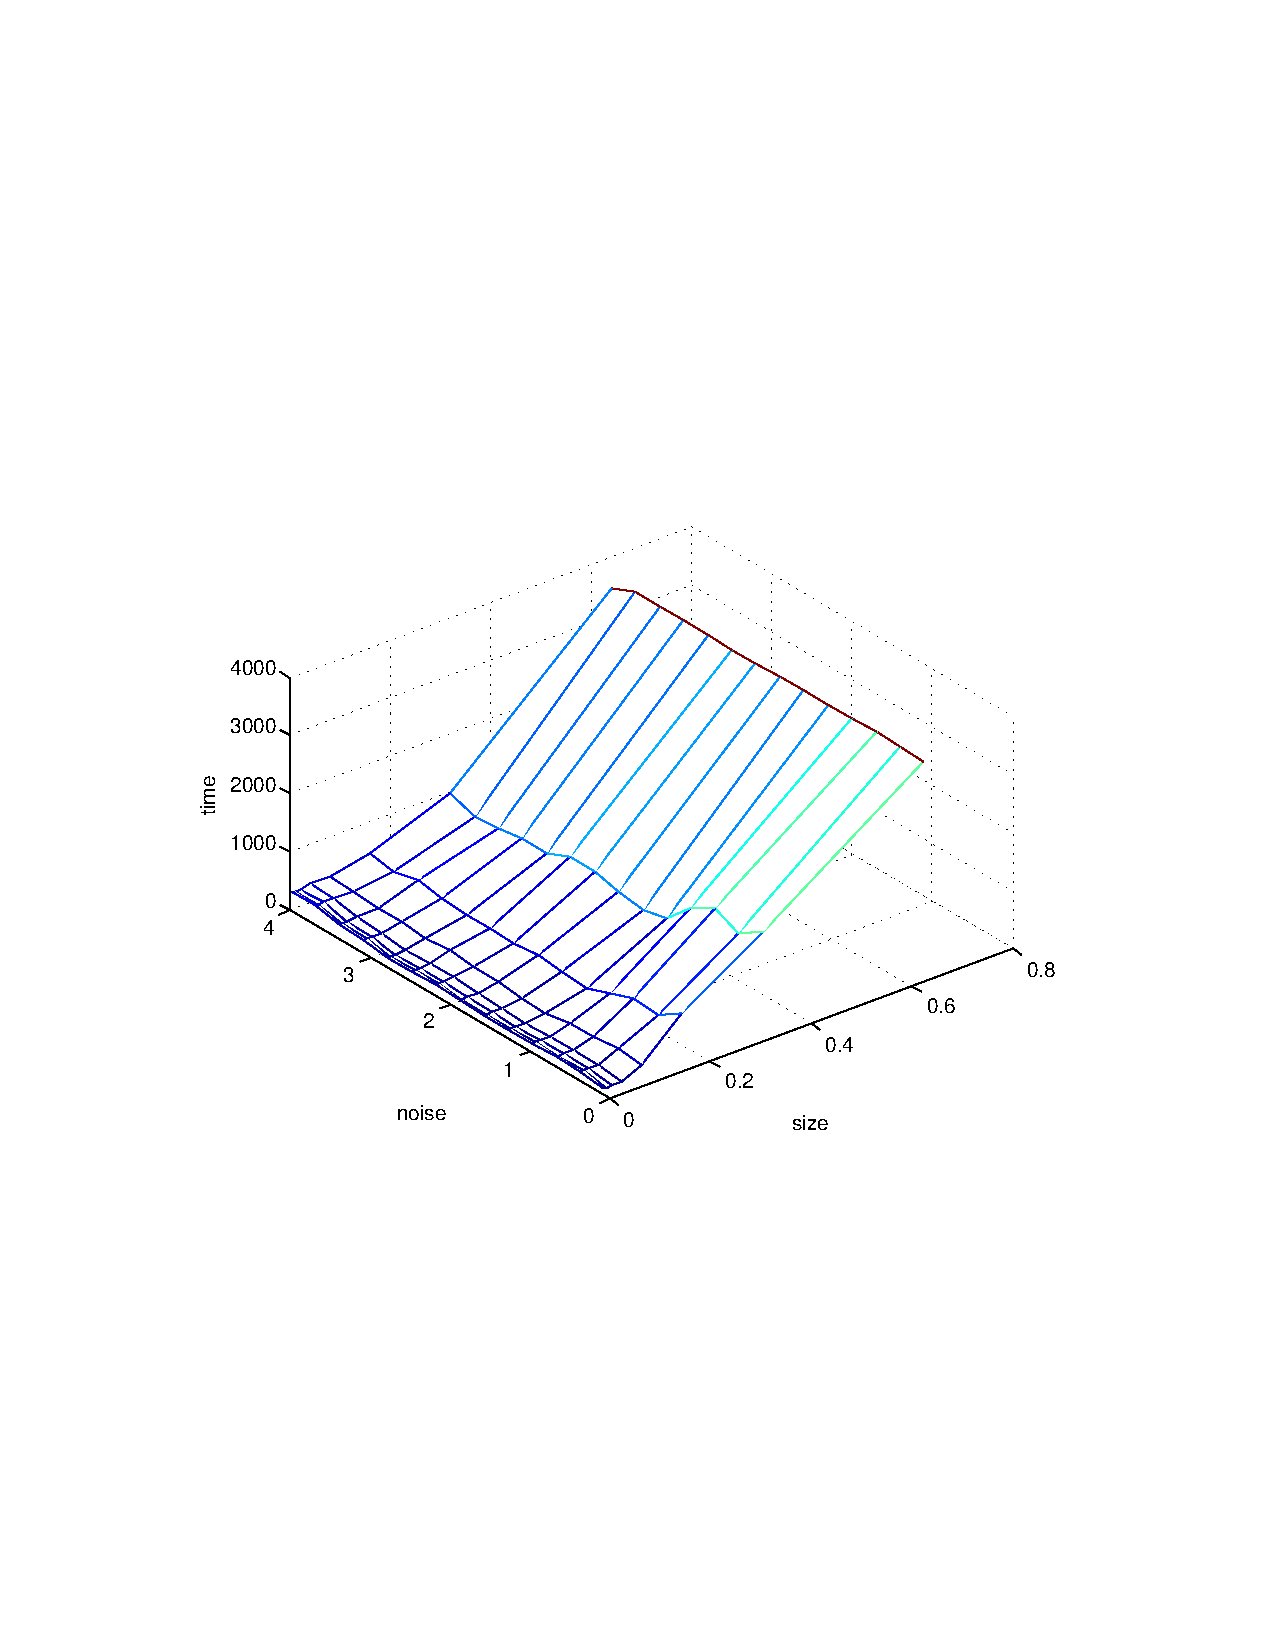
\includegraphics[width=0.45\columnwidth,trim=3.5cm 8cm 4.5cm 8cm,clip]{images/grid-time.pdf}}
\fbox{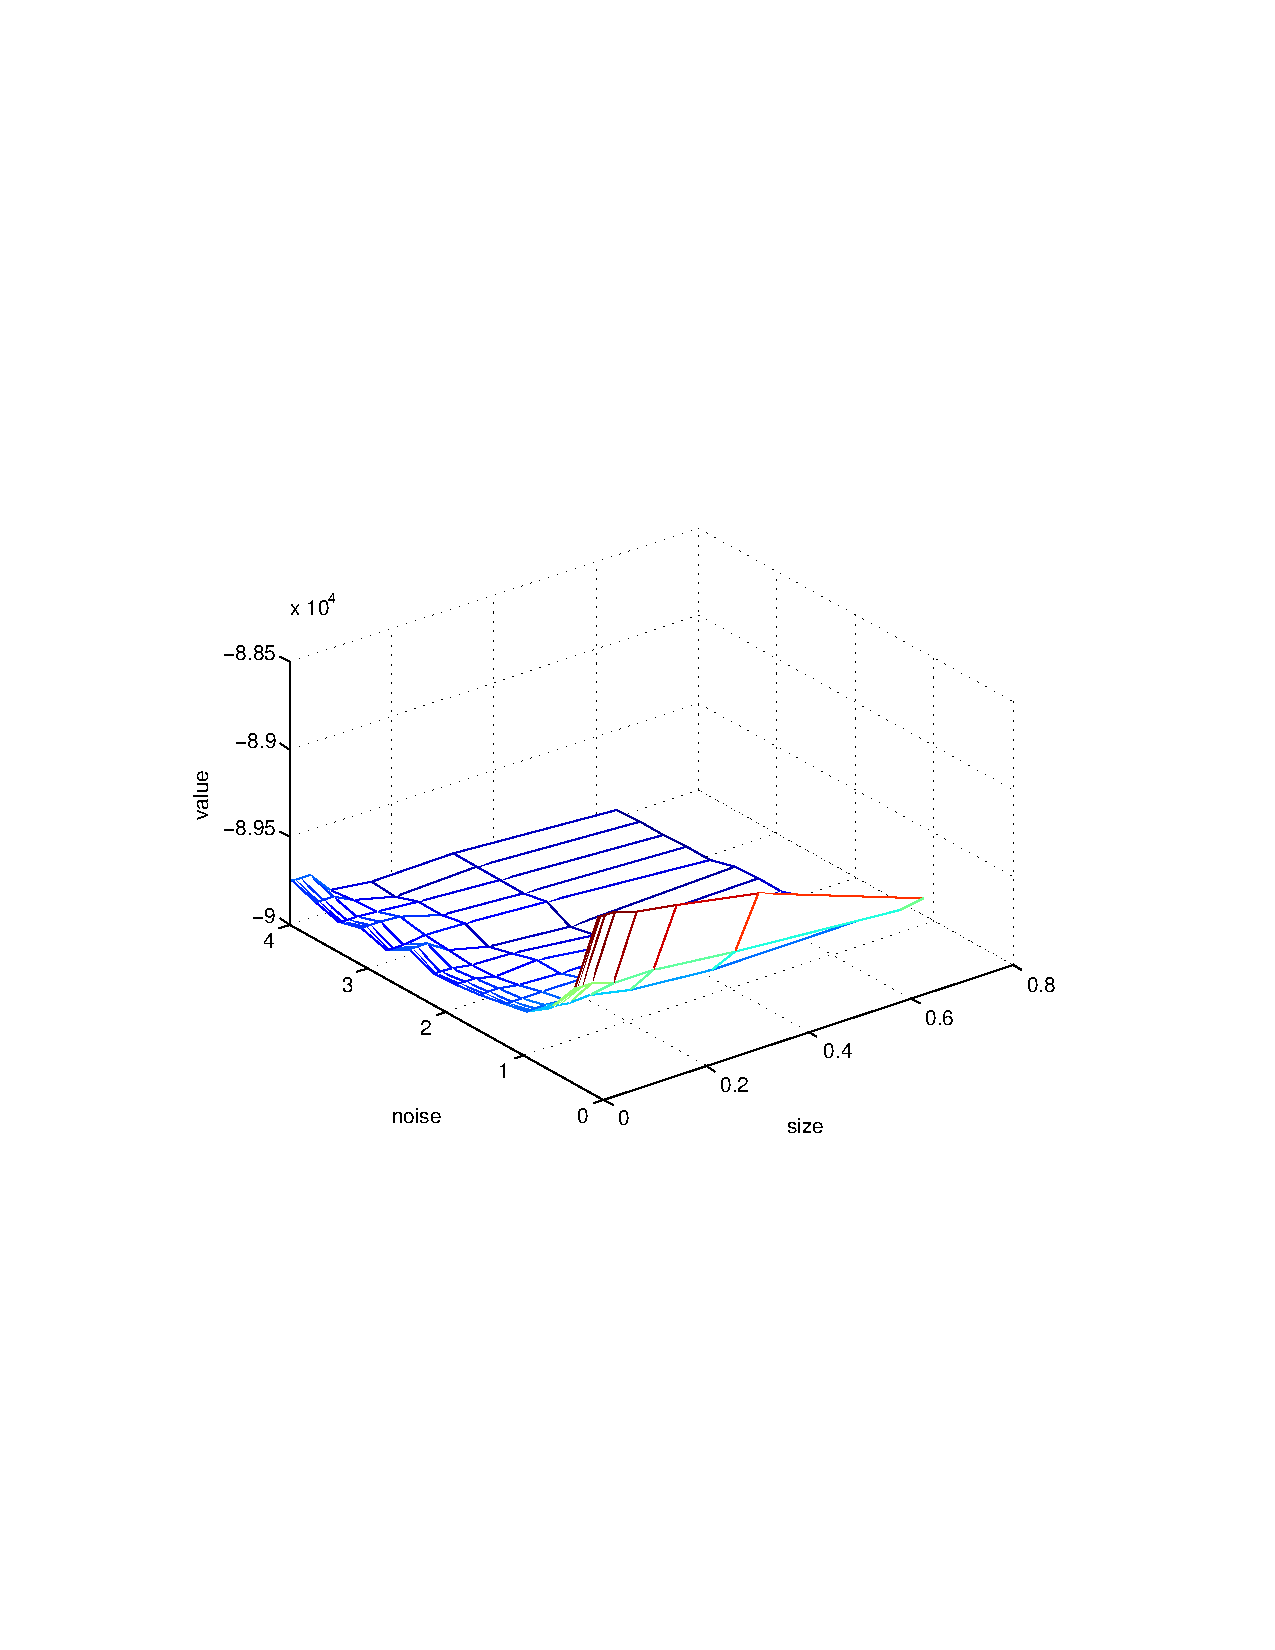
\includegraphics[width=0.45\columnwidth,trim=3.5cm 8cm 4.5cm 8cm,clip]{images/grid-value.pdf}}
\caption{Empirical evaluation of the impact of noise used for proposal generation and proposal size.
  Proposals with many segments causes longer runtime. Noise seemed not to be a critical parameter but should be selected large enough.
}
\end{figure}

\subsection{Benchmark Models}

\newpage
%%%%%%%%%%%%%%%%%%%%%%%%%%%%%%%%%%%%%%%%%%%%%%%%%%%%%%%%%%%%%%%%%%%%%%%%%%%%%%%%%%%%%%%%%%%%
\begin{figure}[p]
\centering
\begin{tikzpicture}
\begin{semilogxaxis}[
restrict y to domain=0:4600,
xlabel = {runtime},
xmin = 0,
xmax = 4100,
%ymin =  75282844.25,
%ymax =  81774642.015,
%xtick       = { 1 , 60 , 3600 },
%xticklabels = { 1 sec. , 1 min.  , 1 hour },
%ytick       = {75661636, 78718140, 81774643 },
%yticklabels = {$75661636$, $78718140$, $81774643$ },
width = 0.9\columnwidth,
scaled ticks = false
]
%\addplot[color=black,mark=x] table[x=time,y=HC-CGC]{data/knott-3d-150.data};
%\addlegendentry{HC-CGC}

\addplot[color=red,mark=x] table[x=time,y=CGC-planar]{data/image-seg.data};
\addlegendentry{CGC-planar} 

\addplot[color=blue,mark=x] table[x=time, y=MCI-CCIFD]{data/image-seg.data};
\addlegendentry{MCI-CCIFD} 

\addplot[color=green,mark=x] table[x=time, y=DYNCC-HC-MC-CGC]{data/image-seg.data};
\addlegendentry{MC-Fusion (HC-MC-CGC)}

\addplot[color=cyan,mark=x] table[x=time, y=DYNCC-HC-CGC-CGC]{data/image-seg.data};
\addlegendentry{MC-Fusion (HC-CGC-CGC)}

\end{semilogxaxis}
\end{tikzpicture}
\caption{image-seg}
\end{figure}
%%%%%%%%%%%%%%%%%%%%%%%%%%%%%%%%%%%%%%%%%%%%%%%%%%%%%%%%%%%%%%%%%%%%%%%%%%%%%%%%%%%%%%%%%%%%%
\begin{figure}[p]
\centering
\begin{tikzpicture}
\begin{semilogxaxis}[
restrict y to domain=-6000:-4500,
xlabel = {runtime},
xmin = 0,
xmax = 4100,
%ymin =  75282844.25,
%ymax =  81774642.015,
%xtick       = { 1 , 60 , 3600 },
%xticklabels = { 1 sec. , 1 min.  , 1 hour },
%ytick       = {75661636, 78718140, 81774643 },
%yticklabels = {$75661636$, $78718140$, $81774643$ },
width = 0.9\columnwidth,
scaled ticks = false
]
%\addplot[color=black,mark=x] table[x=time,y=HC-CGC]{data/knott-3d-150.data};
%\addlegendentry{HC-CGC}

\addplot[color=red,mark=x] table[x=time,y=CGC]{data/knott-3d-150.data};
\addlegendentry{CGC} 

\addplot[color=blue,mark=x] table[x=time, y=MCI-CCIFD]{data/knott-3d-150.data};
\addlegendentry{MCI-CCIFD} 

\addplot[color=green,mark=x] table[x=time, y=DYNCC-HC-MC-CGC]{data/knott-3d-150.data};
\addlegendentry{MC-Fusion (HC-MC-CGC)}

\addplot[color=cyan,mark=x] table[x=time, y=DYNCC-HC-CGC-CGC]{data/knott-3d-150.data};
\addlegendentry{MC-Fusion (HC-CGC-CGC)}

\end{semilogxaxis}
\end{tikzpicture}
\caption{knott-3d-150}
\end{figure}
%%%%%%%%%%%%%%%%%%%%%%%%%%%%%%%%%%%%%%%%%%%%%%%%%%%%%%%%%%%%%%%%%%%%%%%%%%%%%%%%%%%%%%%%%%%%%
\begin{figure}[p]
\centering
\begin{tikzpicture}
\begin{semilogxaxis}[
restrict y to domain=-40000:-24000,
xlabel = {runtime},
xmin = 0,
xmax = 4100,
%ymin =  75282844.25,
%ymax =  81774642.015,
%xtick       = { 1 , 60 , 3600 },
%xticklabels = { 1 sec. , 1 min.  , 1 hour },
%ytick       = {75661636, 78718140, 81774643 },
%yticklabels = {$75661636$, $78718140$, $81774643$ },
width = 0.9\columnwidth,
scaled ticks = false
]
\addplot[color=black,mark=x] table[x=time,y=HC-CGC]{data/knott-3d-300.data};
\addlegendentry{HC-CGC}

\addplot[color=red,mark=x] table[x=time,y=CGC]{data/knott-3d-300.data};
\addlegendentry{CGC} 

\addplot[color=blue,mark=x] table[x=time, y=MCI-CCIFD]{data/knott-3d-300.data};
\addlegendentry{MCI-CCIFD} 

\addplot[color=green,mark=x] table[x=time, y=DYNCC-HC-MC-CGC]{data/knott-3d-300.data};
\addlegendentry{MC-Fusion (HC-MC-CGC)}

\addplot[color=cyan,mark=x] table[x=time, y=DYNCC-HC-CGC-CGC]{data/knott-3d-300.data};
\addlegendentry{MC-Fusion (HC-CGC-CGC)}

\end{semilogxaxis}
\end{tikzpicture}
\caption{knott-3d-300}
\end{figure}
%%%%%%%%%%%%%%%%%%%%%%%%%%%%%%%%%%%%%%%%%%%%%%%%%%%%%%%%%%%%%%%%%%%%%%%%%%%%%%%%%%%%%%%%%%%%%
\begin{figure}[p]
\centering
\begin{tikzpicture}
\begin{semilogxaxis}[
restrict y to domain=-80000:-60000,
xlabel = {runtime},
xmin = 0,
xmax = 4100,
%ymin =  75282844.25,
%ymax =  81774642.015,
%xtick       = { 1 , 60 , 3600 },
%xticklabels = { 1 sec. , 1 min.  , 1 hour },
%ytick       = {75661636, 78718140, 81774643 },
%yticklabels = {$75661636$, $78718140$, $81774643$ },
width = 0.9\columnwidth,
scaled ticks = false
]
\addplot[color=black,mark=x] table[x=time,y=HC-CGC]{data/knott-3d-450.data};
\addlegendentry{HC-CGC}

\addplot[color=red,mark=x] table[x=time,y=CGC]{data/knott-3d-450.data};
\addlegendentry{CGC} 

\addplot[color=blue,mark=x] table[x=time, y=MCI-CCIFD]{data/knott-3d-450.data};
\addlegendentry{MCI-CCIFD} 

\addplot[color=green,mark=x] table[x=time, y=DYNCC-HC-MC-CGC]{data/knott-3d-450.data};
\addlegendentry{MC-Fusion (HC-MC-CGC)}

\addplot[color=cyan,mark=x] table[x=time, y=DYNCC-HC-CGC-CGC]{data/knott-3d-450.data};
\addlegendentry{MC-Fusion (HC-CGC-CGC)}

\end{semilogxaxis}
\end{tikzpicture}
\caption{knott-3d-450}
\end{figure}
%%%%%%%%%%%%%%%%%%%%%%%%%%%%%%%%%%%%%%%%%%%%%%%%%%%%%%%%%%%%%%%%%%%%%%%%%%%%%%%%%%%%%%%%%%%%%
\begin{figure}[p]
\centering
\begin{tikzpicture}
\begin{semilogxaxis}[
restrict y to domain=-10000000:-100000,
xlabel = {runtime},
xmin = 0,
xmax = 4100,
%ymin =  75282844.25,
%ymax =  81774642.015,
%xtick       = { 1 , 60 , 3600 },
%xticklabels = { 1 sec. , 1 min.  , 1 hour },
%ytick       = {75661636, 78718140, 81774643 },
%yticklabels = {$75661636$, $78718140$, $81774643$ },
width = 0.9\columnwidth,
scaled ticks = false
]
\addplot[color=black,mark=x] table[x=time,y=HC-CGC]{data/knott-3d-550.data};
\addlegendentry{HC-CGC}

\addplot[color=red,mark=x] table[x=time,y=CGC]{data/knott-3d-550.data};
\addlegendentry{CGC} 

\addplot[color=blue,mark=x] table[x=time, y=MCI-CCIFD]{data/knott-3d-550.data};
\addlegendentry{MCI-CCIFD} 

\addplot[color=green,mark=x] table[x=time, y=DYNCC-HC-MC-CGC]{data/knott-3d-550.data};
\addlegendentry{MC-Fusion (HC-MC-CGC)}

\addplot[color=cyan,mark=x] table[x=time, y=DYNCC-HC-CGC-CGC]{data/knott-3d-550.data};
\addlegendentry{MC-Fusion (HC-CGC-CGC)}

\end{semilogxaxis}
\end{tikzpicture}
\caption{knott-3d-550}
\end{figure}
%%%%%%%%%%%%%%%%%%%%%%%%%%%%%%%%%%%%%%%%%%%%%%%%%%%%%%%%%%%%%%%%%%%%%%%%%%%%%%%%%%%%%%%%%%%%%\begin{figure}[H]
\begin{figure}[p]
\centering
\begin{tikzpicture}
\begin{semilogxaxis}[
%restrict y to domain=-10000000:-100000,
restrict y to domain=-10000000:700000,
xlabel = {runtime},
xmin = 0,
xmax = 4100,
%ymin =  75282844.25,
%ymax =  81774642.015,
%xtick       = { 1 , 60 , 3600 },
%xticklabels = { 1 sec. , 1 min.  , 1 hour },
%ytick       = {75661636, 78718140, 81774643 },
%yticklabels = {$75661636$, $78718140$, $81774643$ },
width = 0.9\columnwidth,
scaled ticks = false
]
\addplot[color=black,mark=x] table[x=time,y=HC-CGC]{data/seg-3d.data};
\addlegendentry{HC-CGC}

\addplot[color=red,mark=x] table[x=time,y=CGC]{data/seg-3d.data};
\addlegendentry{CGC} 

\addplot[color=blue,mark=x] table[x=time, y=MCI-CCIFD]{data/seg-3d.data};
\addlegendentry{MCI-CCIFD} 

%\addplot[color=yellow,mark=o] table[x=time, y=DYNCC-HC-MC]{data/seg-3d.data};
%\addlegendentry{MC-Fusion (HC-MC)}

\addplot[color=green,mark=o] table[x=time, y=DYNCC-HC-MC-CGC]{data/seg-3d.data};
\addlegendentry{MC-Fusion (HC-MC-CGC)}

\addplot[color=cyan,mark=x] table[x=time, y=DYNCC-HC-CGC-CGC]{data/seg-3d.data};
\addlegendentry{MC-Fusion (HC-CGC-CGC)}

\end{semilogxaxis}
\end{tikzpicture}
\caption{seg-3d}
\end{figure}
%%%%%%%%%%%%%%%%%%%%%%%%%%%%%%%%%%%%%%%%%%%%%%%%%%%%%%%%%%%%%%%%%%%%%%%%%%%%%%%%%%%%%%%%%%%%%



\begin{figure}
\begin{tikzpicture}
  \begin{loglogaxis}[
    xlabel = {runtime},
    ylabel = {distance to optimum/best},
    xlabel style={name=xlabel},
    mark size=1pt,
    every axis/.append style={font=\tiny}, 
    width = 0.95\columnwidth, 
    height= 0.95\columnwidth, 
    legend style = { at={(xlabel.south)}, yshift=-1ex, anchor=north,legend cell align=left, font=\tiny},  
    legend columns = 4 
   ]
  \addplot[only marks, mark=*,red, line width=\thickline,opacity=0.8] table[x=Togm_CGC, y=Vogm_CGC]{\scatterplotpath knott-3d-450.data}; 
  \addlegendentry{CGC};   
 % \addplot[only marks, mark=*,green, line width=\thickline,opacity=0.8] table[x=Togm_HC, y=Vogm_HC]{\scatterplotpath knott-3d-450.data}; 
  %\addlegendentry{HC};   
  \addplot[only marks, mark=*,orange!50, line width=\thickline,opacity=0.8] table[x=Togm_HC_CGC, y=Vogm_HC_CGC]{\scatterplotpath knott-3d-450.data}; 
  \addlegendentry{HC-CGC};   
  %\addplot[only marks, mark=*,cyan, line width=\thickline,opacity=0.8] table[x=Togm_icm, y=Vogm_icm]{\scatterplotpath knott-3d-450.data}; 
  %\addlegendentry{ogm-ICM};   
  \addplot[only marks, mark=*,magenta, line width=\thickline,opacity=0.8] table[x=Togm_kl, y=Vogm_kl]{\scatterplotpath knott-3d-450.data}; 
  \addlegendentry{ogm-KL};   
  %\addplot[only marks, mark=*,black, line width=\thickline,opacity=0.8] table[x=Togm_lf1, y=Vogm_lf1]{\scatterplotpath knott-3d-450.data}; 
  %\addlegendentry{ogm-LF-1};   
  %\addplot[only marks, mark=*,brown, line width=\thickline,opacity=0.8] table[x=Togm_mcfusion_HC_BASE, y=Vogm_mcfusion_HC_BASE]{\scatterplotpath knott-3d-450.data}; 
  %\addlegendentry{DYNCC-HC-B};   
  %\addplot[only marks, mark=*,yellow!70!black, line width=\thickline,opacity=0.8] table[x=Togm_mcfusion_HC_BASE_CGCF, y=Vogm_mcfusion_HC_BASE_CGCF]{\scatterplotpath knott-3d-450.data}; 
  %\addlegendentry{DYNCC-HC-B-CGC};   
  %\addplot[only marks, mark=*,blue!40, line width=\thickline,opacity=0.8] table[x=Togm_mcfusion_HC_CGC, y=Vogm_mcfusion_HC_CGC]{\scatterplotpath knott-3d-450.data}; 
  %\addlegendentry{DYNCC-HC-CGC};   
  \addplot[only marks, mark=*,blue, line width=\thickline,opacity=0.8] table[x=Togm_mcfusion_HC_CGC_CGCF, y=Vogm_mcfusion_HC_CGC_CGCF]{\scatterplotpath knott-3d-450.data}; 
  \addlegendentry{DYNCC-HC-CGC-CGC};   
  %\addplot[only marks, mark=x,red, line width=\thickline,opacity=0.8] table[x=Togm_mcfusion_HC_MC, y=Vogm_mcfusion_HC_MC]{\scatterplotpath knott-3d-450.data}; 
  %\addlegendentry{DYNCC-HC-MC};   
  \addplot[only marks, mark=x,green, line width=\thickline,opacity=0.8] table[x=Togm_mcfusion_HC_MC_CGCF, y=Vogm_mcfusion_HC_MC_CGCF]{\scatterplotpath knott-3d-450.data}; 
  \addlegendentry{DYNCC-HC-MC-CGC};   
  %\addplot[only marks, mark=x,orange!50, line width=\thickline,opacity=0.8] table[x=Togm_mcfusion_WS_BASE, y=Vogm_mcfusion_WS_BASE]{\scatterplotpath knott-3d-450.data}; 
  %\addlegendentry{DYNCC-WS-B};   
  %\addplot[only marks, mark=x,cyan, line width=\thickline,opacity=0.8] table[x=Togm_mcfusion_WS_BASE_CGCF, y=Vogm_mcfusion_WS_BASE_CGCF]{\scatterplotpath knott-3d-450.data}; 
  %\addlegendentry{DYNCC-WS-B-CGC};   
  %\addplot[only marks, mark=x,magenta, line width=\thickline,opacity=0.8] table[x=Togm_mcfusion_WS_CGC, y=Vogm_mcfusion_WS_CGC]{\scatterplotpath knott-3d-450.data}; 
  %\addlegendentry{DYNCC-WS-CGC};   
  %\addplot[only marks, mark=x,black, line width=\thickline,opacity=0.8] table[x=Togm_mcfusion_WS_CGC_CGCF, y=Vogm_mcfusion_WS_CGC_CGCF]{\scatterplotpath knott-3d-450.data}; 
  %\addlegendentry{DYNCC-WS-CGC-CGC};   
  %\addplot[only marks, mark=x,brown, line width=\thickline,opacity=0.8] table[x=Togm_mcfusion_WS_MC, y=Vogm_mcfusion_WS_MC]{\scatterplotpath knott-3d-450.data}; 
  %\addlegendentry{DYNCC-WS-MC};   
  %\addplot[only marks, mark=x,yellow!70!black, line width=\thickline,opacity=0.8] table[x=Togm_mcfusion_WS_MC_CGCF, y=Vogm_mcfusion_WS_MC_CGCF]{\scatterplotpath knott-3d-450.data}; 
  %\addlegendentry{DYNCC-WS-MC-CGC};   
  \addplot[only marks, mark=x,blue!40, line width=\thickline,opacity=0.8] table[x=TMC_CC, y=VMC_CC]{\scatterplotpath knott-3d-450.data}; 
  \addlegendentry{MCR-CC};   
  %\addplot[only marks, mark=x,blue, line width=\thickline,opacity=0.8] table[x=TMC_CCFDB, y=VMC_CCFDB]{\scatterplotpath knott-3d-450.data}; 
  %\addlegendentry{MCR-CCFDB};   
  %\addplot[only marks, mark=square*,red, line width=\thickline,opacity=0.8] table[x=TMC_CCFDB_OWC, y=VMC_CCFDB_OWC]{\scatterplotpath knott-3d-450.data}; 
  %\addlegendentry{MCR-CCFDB-OWC};   
  %\addplot[only marks, mark=square*,green, line width=\thickline,opacity=0.8] table[x=TMC_CCFDB_CCIFD, y=VMC_CCFDB_CCIFD]{\scatterplotpath knott-3d-450.data}; 
  %\addlegendentry{MCI-CCFDB-CCIFD};   
  \addplot[only marks, mark=square*,orange!50, line width=\thickline,opacity=0.8] table[x=TMC_CCI, y=VMC_CCI]{\scatterplotpath knott-3d-450.data}; 
  \addlegendentry{MCI-CCI};   
  \addplot[only marks, mark=square*,cyan, line width=\thickline,opacity=0.8] table[x=TMC_CCIFD, y=VMC_CCIFD]{\scatterplotpath knott-3d-450.data}; 
  \addlegendentry{MCI-CCIFD};   
  \end{loglogaxis} 
\end{tikzpicture} 

\caption{Values and runtime for the 8 knott-3d-450 instances. Note that we use for DYNCC a defensive stopping condition.
A more aggressive one would lead to much faster runtime with only a bit worse values.
DYNCC find solutions with less than distance 100 to the optimum a magnitude faster than the state of the art, which produce poor results on hard instances with a 1 hour time limit.
}
\end{figure}



\subsection{Pixel-wise Multicuts}
%!TEX root = ../egpaper_for_review.tex

\newcounter{cX}
\newcounter{cY}


\newcounter{NPY}
\setcounter{NPY}{30}
\tikzstyle{pixel}=[opacity=1.0,thick,draw opacity=1.0, draw=black]
\tikzstyle{ln}=[opacity=0.6,fill=green,circle,draw, inner sep=0,font=\tiny,minimum size=0.15cm]
\tikzstyle{gn}=[opacity=0.6,fill=red,circle,draw, inner sep=0,font=\tiny,minimum size=0.15cm]
\tikzstyle{p}=[opacity=0.6,fill=white,circle,draw, inner sep=0,font=\tiny,minimum size=0.15cm]
\begin{figure}
\begin{center}
\begin{tikzpicture}[scale=1.0]
    \node[anchor=south west,inner sep=0] (image) at (0,0) 
        {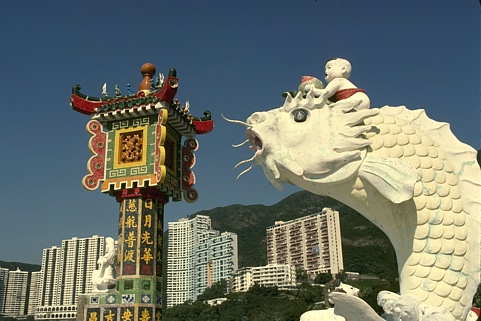
\includegraphics[width=0.4\textwidth]{images/120093.jpg}};
    % shift scope to the image 
    \begin{scope}[x={(image.south east)},y={(image.north west)},xscale=100/481,yscale=100/321]   
        \draw[gray,xstep=3.21/\theNPY, ystep=3.21/\theNPY] (0,0) grid (4.81,3.21);
        % scope of the grid
        \begin{scope}[xscale=3.21/\theNPY,yscale=3.21/\theNPY]  

        \foreach \x\y in {22/18, 10/8} { 
        \setcounter{cX}{\x}
        \setcounter{cY}{\y}
        \draw (\thecX+0.5,\thecY+0.5) node[p]  (centerPixel){};
        \foreach \xx in {-4,0,4} { 
        \foreach \yy in {-4,0,4} { 
            \ifthenelse{\NOT 0 = \xx \OR \NOT 0 = \yy}{
                %\filldraw[green!40!white,pixel] 
                %(\thecX+\xx,\thecY+\yy) rectangle (\thecX+1+\xx,\thecY+1+\yy);
                \draw (\thecX+\xx+0.5,\thecY+\yy+0.5) node[gn](nonLocalPixel){};
                \path[]
                (centerPixel) edge[bend left=0*\xx*\yy ] (nonLocalPixel)
                ;
            }{
            }
        }
        }
        \foreach \xx/\yy/\pColor in {0/1/blue, 0/-1/blue, 1/0/blue, -1/0/blue} { 
            \draw (\thecX+\xx+0.5,\thecY+\yy+0.5) node[ln](nonLocalPixel){};
            (\thecX+\xx,\thecY+\yy) rectangle (\thecX+1+\xx,\thecY+1+\yy);
        }
        }
        % \filldraw[gray,pixel] (\thecX,\thecY) rectangle (\thecX+1,\thecY+1);
        

        \end{scope}
    \end{scope}


\end{tikzpicture}
\end{center}
\caption{
    Pixel Level Multicut:
    every pixel (white nodes) is connected
    to its 4 \emph{local} neighbors (edges between white and green nodes).
    Furthermore each pixel is connected to some \emph{non-local} neighbors within a 
    certain radius  (edges between white and green nodes).
    The local neighbors are connected with a \emph{positive}
    edge weight. If the edge indicator (as gradient magnitude)
    is very high, the local edge weight should be close to zero.
    If there is no evidence for a cut (low gradient magnitude for example)
    the local edge weight should be high.
    The \emph{non-local edge weights} are \emph{negative} to
    encourage label transitions.
    The weight of the non-local edge weights can
    be the negative value of the maximum gradient magnitude
    along a line between the red and white node.
    If there is evidence for a cut between red and white, 
    the weight should be strongly(?) negative.
}
\end{figure}







\section{Conclusion}

    



{\small
\bibliographystyle{ieee}
\bibliography{egbib}
}

\newpage
\onecolumn
\section{Appendix}

\begin{table}[H]
\scriptsize
\centering
\caption{image-seg (100 instances)}
\label{tab:smalltable-image-seg}
\begin{tabular}{lrrrrrr}
\toprule
           algorithm &       runtime     &         value &         bound &           mem &     best &      opt   \\ \midrule 
     ogm-CGC-planar* & $         0.28$ sec & $      4445.22$ & $      4136.83$ & $         0.02$ GB & $      28$ & $       0$ \\ 
ogm-mcfusion-HC-BASE* & $         0.12$ sec & $      5462.60$ & $-\infty$ & $         0.01$ GB & $       0$ & $       0$ \\ 
ogm-mcfusion-HC-BASE-CGCF* & $         0.12$ sec & $      5085.80$ & $-\infty$ & $         0.01$ GB & $       0$ & $       0$ \\ 
ogm-mcfusion-HC-CGC* & $         1.23$ sec & $      4444.56$ & $-\infty$ & $         0.01$ GB & $      40$ & $       0$ \\ 
ogm-mcfusion-HC-CGC-CGCF* & $         1.22$ sec & $      4444.75$ & $-\infty$ & $         0.02$ GB & $      40$ & $       0$ \\ 
 ogm-mcfusion-HC-MC* & $         5.12$ sec & $      4443.61$ & $-\infty$ & $         0.04$ GB & $      73$ & $       0$ \\ 
ogm-mcfusion-HC-MC-CGCF* & $         5.14$ sec & $      4443.61$ & $-\infty$ & $         0.05$ GB & $      73$ & $       0$ \\ 
ogm-mcfusion-WS-BASE* & $         0.05$ sec & $      6622.98$ & $-\infty$ & $         0.01$ GB & $       0$ & $       0$ \\ 
ogm-mcfusion-WS-BASE-CGCF* & $         1.77$ sec & $      4460.12$ & $-\infty$ & $         0.01$ GB & $       3$ & $       0$ \\ 
ogm-mcfusion-WS-CGC* & $         1.44$ sec & $      4445.57$ & $-\infty$ & $         0.01$ GB & $      16$ & $       0$ \\ 
ogm-mcfusion-WS-CGC-CGCF* & $         1.75$ sec & $      4444.59$ & $-\infty$ & $         0.01$ GB & $      27$ & $       0$ \\ 
 ogm-mcfusion-WS-MC* & $         6.00$ sec & $      4444.58$ & $-\infty$ & $         0.03$ GB & $      22$ & $       0$ \\ 
ogm-mcfusion-WS-MC-CGCF* & $         6.31$ sec & $      4443.79$ & $-\infty$ & $         0.03$ GB & $      46$ & $       0$ \\ 
\bottomrule
\end{tabular}
\end{table}
\begin{table}[H]
\scriptsize
\centering
\caption{knott-3d-150 (8 instances)}
\label{tab:anytimetable-knott-3d-150}
\begin{tabular}{lrrrrrrrrrrr}
\toprule
           algorithm &                                   \multicolumn{8}{c}{value} & \multicolumn{1}{c}{time}    & \multicolumn{1}{c}{VI}  & \multicolumn{1}{c}{RI} \\  
\cmidrule(lr){2-9}\cmidrule(lr){10-10} \cmidrule(lr){11-11} \cmidrule(lr){12-12}   
                     & \multicolumn{1}{c}{(0.5 sec)} & \multicolumn{1}{c}{(1 sec)} & \multicolumn{1}{c}{(10 sec)} & \multicolumn{1}{c}{(60 sec)} & \multicolumn{1}{c}{(300 sec)} & \multicolumn{1}{c}{(600 sec)} & \multicolumn{1}{c}{(1800 sec)} & \multicolumn{1}{c}{(end)} & \multicolumn{1}{c}{(end)}    & \multicolumn{1}{c}{(end)}   & \multicolumn{1}{c}{(end)}  \\ \midrule 
          PIVIT-BOEM & $\infty$ & $\infty$ & $      -637.57$ & $      -637.57$ & $      -637.57$ & $      -637.57$ & $      -637.57$ & $      -637.57$ & $         3.01$ sec    & $       2.9936$  & $       0.7851$ \\ 
                 CGC & $     -4566.41$ & $     -4566.41$ & $     -4566.41$ & $     -4566.41$ & $     -4566.41$ & $     -4566.41$ & $     -4566.41$ & $     -4566.41$ & $         0.08$ sec    & $       0.9267$  & $       0.9206$ \\ 
                  HC & $     -3913.60$ & $     -3913.60$ & $     -3913.60$ & $     -3913.60$ & $     -3913.60$ & $     -3913.60$ & $     -3913.60$ & $     -3913.60$ & $         0.01$ sec    & $       1.5477$  & $       0.8139$ \\ 
              HC-CGC & $     -4566.66$ & $     -4566.66$ & $     -4566.66$ & $     -4566.66$ & $     -4566.66$ & $     -4566.66$ & $     -4566.66$ & $     -4566.66$ & $         0.05$ sec    & $       0.9052$  & $       0.9226$ \\ 
              ogm-KL & $     -4431.67$ & $     -4431.67$ & $     -4431.67$ & $     -4431.67$ & $     -4431.67$ & $     -4431.67$ & $     -4431.67$ & $     -4431.67$ & $         0.12$ sec    & $       2.0648$  & $       0.8085$ \\ 
    CC-Fusion-HC-CGC & $     -4557.70$ & $     -4558.80$ & $     -4558.80$ & $     -4558.80$ & $     -4558.80$ & $     -4558.80$ & $     -4558.80$ & $     -4558.80$ & $         0.56$ sec    & $       0.9679$  & $       0.9031$ \\ 
     CC-Fusion-HC-MC & $     -4558.98$ & $     -4559.96$ & $     -4559.96$ & $     -4559.96$ & $     -4559.96$ & $     -4559.96$ & $     -4559.96$ & $     -4559.96$ & $         1.72$ sec    & $       0.9629$  & $       0.9042$ \\ 
    CC-Fusion-WS-CGC & $     -4548.38$ & $     -4548.38$ & $     -4548.38$ & $     -4548.38$ & $     -4548.38$ & $     -4548.38$ & $     -4548.38$ & $     -4548.38$ & $         0.44$ sec    & $       1.0585$  & $       0.8951$ \\ 
     CC-Fusion-WS-MC & $     -4549.12$ & $     -4559.19$ & $     -4559.96$ & $     -4559.96$ & $     -4559.96$ & $     -4559.96$ & $     -4559.96$ & $     -4559.96$ & $         3.48$ sec    & $       0.9629$  & $       0.9042$ \\ 
\cmidrule{1-1} 
           MCR-CCFDB & $     -4165.54$ & $     -4544.50$ & $     -4568.94$ & $     -4568.94$ & $     -4568.94$ & $     -4568.94$ & $     -4568.94$ & $     -4568.94$ & $         0.63$ sec    & $       0.9178$  & $       0.9232$ \\ 
\cmidrule{1-1} 
           MCI-CCIFD & $     -4487.83$ & $     -4571.69$ & $     -4571.69$ & $     -4571.69$ & $     -4571.69$ & $     -4571.69$ & $     -4571.69$ & $     -4571.69$ & $         0.48$ sec    & $       0.9063$  & $       0.9236$ \\ 
\bottomrule
\end{tabular}
\end{table}
\begin{table}[H]
\scriptsize
\centering
\caption{knott-3d-300 (8 instances)}
\label{tab:anytimetable-knott-3d-300}
\begin{tabular}{lrrrrrrr}
\toprule
           algorithm &                                   \multicolumn{6}{c}{value} & \multicolumn{1}{c}{time}   \\  
\cmidrule(lr){2-7}\cmidrule(lr){8-8}  
                     & \multicolumn{1}{c}{(1 sec)} & \multicolumn{1}{c}{(10 sec)} & \multicolumn{1}{c}{(60 sec)} & \multicolumn{1}{c}{(600 sec)} & \multicolumn{1}{c}{(1800 sec)} & \multicolumn{1}{c}{(end)} & \multicolumn{1}{c}{(end)}   \\ \midrule 
                 CGC & $     -5347.53$ & $    -27251.42$ & $    -27251.42$ & $    -27251.42$ & $    -27251.42$ & $    -27251.42$ & $         5.95$ sec   \\ 
                  HC & $    -24120.16$ & $    -24120.16$ & $    -24120.16$ & $    -24120.16$ & $    -24120.16$ & $    -24120.16$ & $         0.06$ sec   \\ 
              HC-CGC & $    -26090.18$ & $    -26090.18$ & $    -26090.18$ & $    -26090.18$ & $    -26090.18$ & $    -26090.18$ & $         0.10$ sec   \\ 
             ogm-ICM & $         0.00$ & $      -632.20$ & $     -2311.81$ & $    -25196.51$ & $    -25196.51$ & $    -25196.51$ & $        83.87$ sec   \\ 
              ogm-KL & $     -1989.98$ & $    -25553.07$ & $    -25556.93$ & $    -25556.93$ & $    -25556.93$ & $    -25556.93$ & $        12.72$ sec   \\ 
            ogm-LF-1 & $     -2001.60$ & $    -17394.47$ & $    -25243.76$ & $    -25243.76$ & $    -25243.76$ & $    -25243.76$ & $        30.36$ sec   \\ 
          DYNCC-HC-B & $    -22041.99$ & $    -22347.85$ & $    -22347.85$ & $    -22347.85$ & $    -22347.85$ & $    -22347.85$ & $         2.63$ sec   \\ 
      DYNCC-HC-B-CGC & $    -22091.11$ & $    -24683.70$ & $    -24683.70$ & $    -24683.70$ & $    -24683.70$ & $    -24683.70$ & $         2.63$ sec   \\ 
        DYNCC-HC-CGC & $    -27136.08$ & $    -27244.54$ & $    -27244.54$ & $    -27244.54$ & $    -27244.54$ & $    -27244.54$ & $         6.60$ sec   \\ 
    DYNCC-HC-CGC-CGC & $    -27185.66$ & $    -27283.82$ & $    -27283.82$ & $    -27283.82$ & $    -27283.82$ & $    -27283.82$ & $         6.51$ sec   \\ 
         DYNCC-HC-MC & $    -23976.49$ & $    -27198.66$ & $    -27283.36$ & $    -27283.36$ & $    -27283.36$ & $    -27283.36$ & $        35.87$ sec   \\ 
     DYNCC-HC-MC-CGC & $    -22764.91$ & $    -27195.11$ & $    -27284.60$ & $    -27284.60$ & $    -27284.60$ & $    -27284.60$ & $        36.75$ sec   \\ 
          DYNCC-WS-B & $     -8146.11$ & $     -8146.11$ & $     -8146.11$ & $     -8146.11$ & $     -8146.11$ & $     -8146.11$ & $         0.63$ sec   \\ 
      DYNCC-WS-B-CGC & $    -14280.11$ & $    -25673.33$ & $    -25674.01$ & $    -25674.01$ & $    -25674.01$ & $    -25674.01$ & $         6.37$ sec   \\ 
        DYNCC-WS-CGC & $    -23319.45$ & $    -27249.34$ & $    -27274.74$ & $    -27274.74$ & $    -27274.74$ & $    -27274.74$ & $        26.42$ sec   \\ 
    DYNCC-WS-CGC-CGC & $    -23319.45$ & $    -27249.92$ & $    -27287.98$ & $    -27287.98$ & $    -27287.98$ & $    -27287.98$ & $        27.36$ sec   \\ 
         DYNCC-WS-MC & $     -6750.17$ & $    -23748.04$ & $    -27270.11$ & $    -27280.59$ & $    -27280.59$ & $    -27280.59$ & $        71.37$ sec   \\ 
     DYNCC-WS-MC-CGC & $     -6750.17$ & $    -24876.03$ & $    -27270.72$ & $    -27293.33$ & $    -27293.33$ & $    -27293.33$ & $        72.57$ sec   \\ 
\cmidrule{1-1} 
              MCR-CC & $     -1989.98$ & $     -1989.98$ & $    -18165.98$ & $    -27279.61$ & $    -27289.63$ & $    -27289.63$ & $       511.21$ sec   \\ 
           MCR-CCFDB & $     -1989.98$ & $     -1989.98$ & $    -14242.47$ & $    -27289.63$ & $    -27289.63$ & $    -27289.63$ & $       229.98$ sec   \\ 
       MCR-CCFDB-OWC & $     -1989.98$ & $     -2297.81$ & $    -12974.38$ & $    -27300.22$ & $    -27300.22$ & $    -27300.22$ & $       205.71$ sec   \\ 
\cmidrule{1-1} 
     MCI-CCFDB-CCIFD & $     -1989.98$ & $     -2239.37$ & $    -15517.93$ & $    -27302.78$ & $    -27302.78$ & $    -27302.78$ & $       194.30$ sec   \\ 
             MCI-CCI & $     -1989.98$ & $    -23227.40$ & $    -27257.36$ & $    -27290.39$ & $    -27302.78$ & $    -27302.78$ & $       207.03$ sec   \\ 
           MCI-CCIFD & $     -1989.98$ & $    -23344.27$ & $    -27290.36$ & $    -27302.78$ & $    -27302.78$ & $    -27302.78$ & $        47.30$ sec   \\ 
\bottomrule
\end{tabular}
\end{table}
\begin{tikzpicture}
  \begin{loglogaxis}[
    xlabel = {runtime},
    ylabel = {distance to optimum/best},
    xlabel style={name=xlabel},
    mark size=1pt,
    every axis/.append style={font=\tiny}, 
    width = 0.95\columnwidth, 
    height= 0.95\columnwidth, 
    legend style = { at={(xlabel.south)}, yshift=-1ex, anchor=north,legend cell align=left, font=\tiny},  
    legend columns = 4 
   ]
  \addplot[only marks, mark=*,red, line width=\thickline,opacity=0.8] table[x=Togm_CGC, y=Vogm_CGC]{\scatterplotpath knott-3d-450.data}; 
  \addlegendentry{CGC};   
 % \addplot[only marks, mark=*,green, line width=\thickline,opacity=0.8] table[x=Togm_HC, y=Vogm_HC]{\scatterplotpath knott-3d-450.data}; 
  %\addlegendentry{HC};   
  \addplot[only marks, mark=*,orange!50, line width=\thickline,opacity=0.8] table[x=Togm_HC_CGC, y=Vogm_HC_CGC]{\scatterplotpath knott-3d-450.data}; 
  \addlegendentry{HC-CGC};   
  %\addplot[only marks, mark=*,cyan, line width=\thickline,opacity=0.8] table[x=Togm_icm, y=Vogm_icm]{\scatterplotpath knott-3d-450.data}; 
  %\addlegendentry{ogm-ICM};   
  \addplot[only marks, mark=*,magenta, line width=\thickline,opacity=0.8] table[x=Togm_kl, y=Vogm_kl]{\scatterplotpath knott-3d-450.data}; 
  \addlegendentry{ogm-KL};   
  %\addplot[only marks, mark=*,black, line width=\thickline,opacity=0.8] table[x=Togm_lf1, y=Vogm_lf1]{\scatterplotpath knott-3d-450.data}; 
  %\addlegendentry{ogm-LF-1};   
  %\addplot[only marks, mark=*,brown, line width=\thickline,opacity=0.8] table[x=Togm_mcfusion_HC_BASE, y=Vogm_mcfusion_HC_BASE]{\scatterplotpath knott-3d-450.data}; 
  %\addlegendentry{DYNCC-HC-B};   
  %\addplot[only marks, mark=*,yellow!70!black, line width=\thickline,opacity=0.8] table[x=Togm_mcfusion_HC_BASE_CGCF, y=Vogm_mcfusion_HC_BASE_CGCF]{\scatterplotpath knott-3d-450.data}; 
  %\addlegendentry{DYNCC-HC-B-CGC};   
  %\addplot[only marks, mark=*,blue!40, line width=\thickline,opacity=0.8] table[x=Togm_mcfusion_HC_CGC, y=Vogm_mcfusion_HC_CGC]{\scatterplotpath knott-3d-450.data}; 
  %\addlegendentry{DYNCC-HC-CGC};   
  \addplot[only marks, mark=*,blue, line width=\thickline,opacity=0.8] table[x=Togm_mcfusion_HC_CGC_CGCF, y=Vogm_mcfusion_HC_CGC_CGCF]{\scatterplotpath knott-3d-450.data}; 
  \addlegendentry{DYNCC-HC-CGC-CGC};   
  %\addplot[only marks, mark=x,red, line width=\thickline,opacity=0.8] table[x=Togm_mcfusion_HC_MC, y=Vogm_mcfusion_HC_MC]{\scatterplotpath knott-3d-450.data}; 
  %\addlegendentry{DYNCC-HC-MC};   
  \addplot[only marks, mark=x,green, line width=\thickline,opacity=0.8] table[x=Togm_mcfusion_HC_MC_CGCF, y=Vogm_mcfusion_HC_MC_CGCF]{\scatterplotpath knott-3d-450.data}; 
  \addlegendentry{DYNCC-HC-MC-CGC};   
  %\addplot[only marks, mark=x,orange!50, line width=\thickline,opacity=0.8] table[x=Togm_mcfusion_WS_BASE, y=Vogm_mcfusion_WS_BASE]{\scatterplotpath knott-3d-450.data}; 
  %\addlegendentry{DYNCC-WS-B};   
  %\addplot[only marks, mark=x,cyan, line width=\thickline,opacity=0.8] table[x=Togm_mcfusion_WS_BASE_CGCF, y=Vogm_mcfusion_WS_BASE_CGCF]{\scatterplotpath knott-3d-450.data}; 
  %\addlegendentry{DYNCC-WS-B-CGC};   
  %\addplot[only marks, mark=x,magenta, line width=\thickline,opacity=0.8] table[x=Togm_mcfusion_WS_CGC, y=Vogm_mcfusion_WS_CGC]{\scatterplotpath knott-3d-450.data}; 
  %\addlegendentry{DYNCC-WS-CGC};   
  %\addplot[only marks, mark=x,black, line width=\thickline,opacity=0.8] table[x=Togm_mcfusion_WS_CGC_CGCF, y=Vogm_mcfusion_WS_CGC_CGCF]{\scatterplotpath knott-3d-450.data}; 
  %\addlegendentry{DYNCC-WS-CGC-CGC};   
  %\addplot[only marks, mark=x,brown, line width=\thickline,opacity=0.8] table[x=Togm_mcfusion_WS_MC, y=Vogm_mcfusion_WS_MC]{\scatterplotpath knott-3d-450.data}; 
  %\addlegendentry{DYNCC-WS-MC};   
  %\addplot[only marks, mark=x,yellow!70!black, line width=\thickline,opacity=0.8] table[x=Togm_mcfusion_WS_MC_CGCF, y=Vogm_mcfusion_WS_MC_CGCF]{\scatterplotpath knott-3d-450.data}; 
  %\addlegendentry{DYNCC-WS-MC-CGC};   
  \addplot[only marks, mark=x,blue!40, line width=\thickline,opacity=0.8] table[x=TMC_CC, y=VMC_CC]{\scatterplotpath knott-3d-450.data}; 
  \addlegendentry{MCR-CC};   
  %\addplot[only marks, mark=x,blue, line width=\thickline,opacity=0.8] table[x=TMC_CCFDB, y=VMC_CCFDB]{\scatterplotpath knott-3d-450.data}; 
  %\addlegendentry{MCR-CCFDB};   
  %\addplot[only marks, mark=square*,red, line width=\thickline,opacity=0.8] table[x=TMC_CCFDB_OWC, y=VMC_CCFDB_OWC]{\scatterplotpath knott-3d-450.data}; 
  %\addlegendentry{MCR-CCFDB-OWC};   
  %\addplot[only marks, mark=square*,green, line width=\thickline,opacity=0.8] table[x=TMC_CCFDB_CCIFD, y=VMC_CCFDB_CCIFD]{\scatterplotpath knott-3d-450.data}; 
  %\addlegendentry{MCI-CCFDB-CCIFD};   
  \addplot[only marks, mark=square*,orange!50, line width=\thickline,opacity=0.8] table[x=TMC_CCI, y=VMC_CCI]{\scatterplotpath knott-3d-450.data}; 
  \addlegendentry{MCI-CCI};   
  \addplot[only marks, mark=square*,cyan, line width=\thickline,opacity=0.8] table[x=TMC_CCIFD, y=VMC_CCIFD]{\scatterplotpath knott-3d-450.data}; 
  \addlegendentry{MCI-CCIFD};   
  \end{loglogaxis} 
\end{tikzpicture} 

\begin{table}[H]
\scriptsize
\centering
\caption{knott-3d-550 (8 instances)}
\label{tab:anytimetable-knott-3d-550}
\begin{tabular}{lrrrrrrr}
\toprule
           algorithm &                                   \multicolumn{6}{c}{value} & \multicolumn{1}{c}{time}   \\  
\cmidrule(lr){2-7}\cmidrule(lr){8-8}  
                     & \multicolumn{1}{c}{(1 sec)} & \multicolumn{1}{c}{(10 sec)} & \multicolumn{1}{c}{(60 sec)} & \multicolumn{1}{c}{(600 sec)} & \multicolumn{1}{c}{(1800 sec)} & \multicolumn{1}{c}{(end)} & \multicolumn{1}{c}{(end)}   \\ \midrule 
                 CGC & $     -2794.65$ & $     -2794.65$ & $    -14877.47$ & $   -136069.76$ & $   -136188.55$ & $   -136188.55$ & $       600.91$ sec   \\ 
                  HC & $   -119817.00$ & $   -119817.00$ & $   -119817.00$ & $   -119817.00$ & $   -119817.00$ & $   -119817.00$ & $         0.74$ sec   \\ 
              HC-CGC & $   -121631.47$ & $   -129298.08$ & $   -129298.08$ & $   -129298.08$ & $   -129298.08$ & $   -129298.08$ & $         2.24$ sec   \\ 
             ogm-ICM & $         0.00$ & $         0.00$ & $         0.00$ & $         0.00$ & $         0.00$ & $   -126335.53$ & $      2792.82$ sec   \\ 
              ogm-KL & $     -8187.14$ & $     -8187.14$ & $     -8187.14$ & $   -127030.98$ & $   -127032.70$ & $   -127032.70$ & $       607.99$ sec   \\ 
            ogm-LF-1 & $         0.00$ & $         0.00$ & $         0.00$ & $         0.00$ & $   -126356.35$ & $   -126356.35$ & $       987.13$ sec   \\ 
          DYNCC-HC-B & $    -98305.49$ & $   -103055.28$ & $   -104061.64$ & $   -104061.64$ & $   -104061.64$ & $   -104061.64$ & $        26.82$ sec   \\ 
      DYNCC-HC-B-CGC & $    -97043.55$ & $   -103055.28$ & $   -116531.68$ & $   -116531.68$ & $   -116531.68$ & $   -116531.68$ & $        30.28$ sec   \\ 
        DYNCC-HC-CGC & $    -86863.93$ & $   -128703.18$ & $   -136411.54$ & $   -136470.59$ & $   -136470.59$ & $   -136470.59$ & $       227.83$ sec   \\ 
    DYNCC-HC-CGC-CGC & $    -86863.93$ & $   -128524.40$ & $   -136403.32$ & $   -136479.42$ & $   -136479.42$ & $   -136479.42$ & $       238.92$ sec   \\ 
         DYNCC-HC-MC & $    -86863.93$ & $   -117685.52$ & $   -136280.38$ & $   -136449.81$ & $   -136449.81$ & $   -136449.81$ & $       358.68$ sec   \\ 
     DYNCC-HC-MC-CGC & $    -86863.93$ & $   -117685.52$ & $   -136274.41$ & $   -136468.45$ & $   -136468.45$ & $   -136468.45$ & $       375.73$ sec   \\ 
          DYNCC-WS-B & $      -536.76$ & $     -1567.84$ & $     -1567.84$ & $     -1567.84$ & $     -1567.84$ & $     -1567.84$ & $         5.82$ sec   \\ 
      DYNCC-WS-B-CGC & $         0.00$ & $         0.00$ & $         0.00$ & $    -69442.33$ & $   -136316.11$ & $   -136316.11$ & $       751.01$ sec   \\ 
        DYNCC-WS-CGC & $      -329.88$ & $      -329.88$ & $    -71141.29$ & $   -136382.93$ & $   -136453.83$ & $   -136456.60$ & $      1789.22$ sec   \\ 
    DYNCC-WS-CGC-CGC & $      -329.88$ & $      -329.88$ & $    -69376.98$ & $   -136381.99$ & $   -136470.18$ & $   -136494.75$ & $      1969.54$ sec   \\ 
         DYNCC-WS-MC & $      -329.88$ & $      -329.88$ & $    -33748.48$ & $   -136450.05$ & $   -136506.95$ & $   -136507.19$ & $      1662.88$ sec   \\ 
     DYNCC-WS-MC-CGC & $      -329.88$ & $      -329.88$ & $    -15941.49$ & $   -136444.59$ & $   -136511.97$ & $   -136525.35$ & $      1840.19$ sec   \\ 
\cmidrule{1-1} 
              MCR-CC & $     -8187.14$ & $     -8187.14$ & $     -8187.14$ & $     -8187.14$ & $    -36907.88$ & $    -81210.53$ & $      3953.04$ sec   \\ 
           MCR-CCFDB & $     -8187.14$ & $     -8187.14$ & $     -8187.14$ & $     -8187.14$ & $    -34931.99$ & $    -69360.14$ & $      3764.81$ sec   \\ 
       MCR-CCFDB-OWC & $     -8187.14$ & $     -8187.14$ & $     -8187.14$ & $     -8974.82$ & $    -36297.50$ & $    -72149.80$ & $      3759.50$ sec   \\ 
\cmidrule{1-1} 
     MCI-CCFDB-CCIFD & $     -8187.14$ & $     -8187.14$ & $     -8187.14$ & $    -12045.79$ & $    -36297.50$ & $    -73678.41$ & $      3762.01$ sec   \\ 
             MCI-CCI & $     -8187.14$ & $     -8187.14$ & $     -8187.14$ & $    -91478.44$ & $   -135274.80$ & $   -135752.76$ & $      3546.74$ sec   \\ 
           MCI-CCIFD & $     -8187.14$ & $     -8187.14$ & $     -8187.14$ & $    -78689.15$ & $   -136191.79$ & $   -136321.25$ & $      2512.74$ sec   \\ 
\bottomrule
\end{tabular}
\end{table}
\begin{table}[H]
\tiny
\centering
\caption{seg-3d (2 instances)}
\label{tab:anytimetable-seg-3d}
\begin{tabular}{lrrrrrrr}
\toprule
           algorithm &                                   \multicolumn{6}{c}{value} & \multicolumn{1}{c}{time}   \\  
\cmidrule(lr){2-7}\cmidrule(lr){8-8}  
                     & \multicolumn{1}{c}{(1 sec)} & \multicolumn{1}{c}{(10 sec)} & \multicolumn{1}{c}{(60 sec)} & \multicolumn{1}{c}{(600 sec)} & \multicolumn{1}{c}{(1800 sec)} & \multicolumn{1}{c}{(end)} & \multicolumn{1}{c}{(end)}   \\ \midrule 
                 CGC & $    695060.64$ & $    664862.46$ & $    664862.46$ & $    664862.46$ & $    498966.33$ & $    441683.29$ & $      1807.93$ sec   \\ 
                  HC & $    434733.18$ & $    434733.18$ & $    434733.18$ & $    434733.18$ & $    434733.18$ & $    434733.18$ & $         0.90$ sec   \\ 
              HC-CGC & $\infty$ & $\infty$ & $\infty$ & $\infty$ & $\infty$ & $          NaN$ & $          NaN$ sec   \\ 
             ogm-ICM & $    745275.57$ & $    745275.57$ & $    745275.57$ & $    666581.09$ & $    666581.09$ & $    618528.21$ & $      1960.01$ sec   \\ 
              ogm-KL & $    691974.89$ & $    691974.89$ & $    654696.62$ & $    654696.62$ & $    654696.62$ & $    441695.84$ & $      2787.12$ sec   \\ 
            ogm-LF-1 & $    745275.57$ & $    745275.57$ & $    745275.57$ & $    666584.62$ & $    666584.62$ & $    553739.77$ & $      1857.03$ sec   \\ 
          DYNCC-HC-B & $    500696.18$ & $    479494.65$ & $    479112.62$ & $    479112.62$ & $    479112.62$ & $    479112.62$ & $        51.17$ sec   \\ 
      DYNCC-HC-B-CGC & $    668158.52$ & $    477220.61$ & $    476838.57$ & $    450526.86$ & $    450526.86$ & $    450526.86$ & $        73.40$ sec   \\ 
        DYNCC-HC-CGC & $    664869.17$ & $    497382.76$ & $    414338.79$ & $    413587.54$ & $    413560.35$ & $    413549.46$ & $      1474.91$ sec   \\ 
    DYNCC-HC-CGC-CGC & $    664869.17$ & $    497382.76$ & $    414528.86$ & $    413587.54$ & $    413560.57$ & $    413549.44$ & $      1494.97$ sec   \\ 
         DYNCC-HC-MC & $    497406.71$ & $    497382.95$ & $    415370.46$ & $    413597.88$ & $    413552.95$ & $    413552.74$ & $      1273.57$ sec   \\ 
     DYNCC-HC-MC-CGC & $    664869.05$ & $    497382.95$ & $    415370.46$ & $    413597.88$ & $    413552.95$ & $    413546.96$ & $      1272.86$ sec   \\ 
          DYNCC-WS-B & $    685915.55$ & $    685915.55$ & $    685915.55$ & $    685915.55$ & $    685915.55$ & $    685915.55$ & $        16.84$ sec   \\ 
      DYNCC-WS-B-CGC & $    745275.57$ & $    664860.06$ & $    664860.06$ & $    664860.06$ & $    664860.06$ & $    434904.61$ & $      1802.69$ sec   \\ 
        DYNCC-WS-CGC & $    665629.81$ & $    664857.82$ & $    664847.04$ & $    664847.04$ & $    664847.04$ & $    428682.14$ & $      2027.00$ sec   \\ 
    DYNCC-WS-CGC-CGC & $    665629.81$ & $    664857.82$ & $    664845.10$ & $    664845.10$ & $    664845.10$ & $    428575.34$ & $      2053.05$ sec   \\ 
         DYNCC-WS-MC & $    665973.32$ & $    664863.35$ & $    664846.57$ & $    416174.04$ & $    413746.63$ & $    413653.88$ & $      1842.91$ sec   \\ 
     DYNCC-WS-MC-CGC & $    665973.32$ & $    664863.35$ & $    664844.71$ & $    416172.18$ & $    413744.77$ & $    413643.31$ & $      1839.70$ sec   \\ 
\cmidrule{1-1} 
              MCR-CC & $    681113.67$ & $    681113.67$ & $    650888.58$ & $    650888.58$ & $    650888.58$ & $    650888.58$ & $      8084.96$ sec   \\ 
           MCR-CCFDB & $    681113.67$ & $    681113.67$ & $    650888.58$ & $    650888.58$ & $    650888.58$ & $    650888.58$ & $      3948.26$ sec   \\ 
       MCR-CCFDB-OWC & $    681113.67$ & $    681113.67$ & $    650888.58$ & $    650888.58$ & $    650888.58$ & $    650888.58$ & $      4074.76$ sec   \\ 
\cmidrule{1-1} 
     MCI-CCFDB-CCIFD & $    681113.67$ & $    681113.67$ & $    650888.58$ & $    650888.58$ & $    650888.58$ & $    650888.58$ & $      4021.04$ sec   \\ 
             MCI-CCI & $    681113.67$ & $    650927.43$ & $    650888.58$ & $    599966.22$ & $    534464.79$ & $    414563.99$ & $      1807.90$ sec   \\ 
           MCI-CCIFD & $    681113.67$ & $    650918.38$ & $    650888.58$ & $    606644.77$ & $    505587.24$ & $    413722.38$ & $      1814.62$ sec   \\ 
\bottomrule
\end{tabular}
\end{table}

\begin{table}[H]
\scriptsize
\centering
\caption{modularity-clustering (6 instances)}
\label{tab:smalltable-modularity-clustering}
\begin{tabular}{lrrrrrr}
\toprule
           algorithm &       runtime     &         value &         bound &           mem &     best &      opt   \\ \midrule 
             ogm-ICM & $         0.09$ sec & $       0.0000$ & $-\infty$ & $         0.01$ GB & $       0$ & $       0$ \\ 
              ogm-KL & $         0.01$ sec & $      -0.4860$ & $-\infty$ & $         0.01$ GB & $       3$ & $       0$ \\ 
            ogm-LF-1 & $         0.03$ sec & $       0.0000$ & $-\infty$ & $         0.01$ GB & $       0$ & $       0$ \\ 
\cmidrule{1-1} 
              MCR-CC & $        97.63$ sec & $      -0.4543$ & $      -0.5094$ & $         0.14$ GB & $       2$ & $       1$ \\ 
           MCR-CCFDB & $         1.81$ sec & $      -0.4543$ & $      -0.5094$ & $         0.03$ GB & $       1$ & $       1$ \\ 
       MCR-CCFDB-OWC & $       602.50$ sec & $      -0.4652$ & $      -0.4962$ & $         0.03$ GB & $       5$ & $       5$ \\ 
\cmidrule{1-1} 
     MCI-CCFDB-CCIFD & $       601.28$ sec & $      -0.4537$ & $      -0.5021$ & $         1.85$ GB & $       5$ & $       5$ \\ 
             MCI-CCI & $      1206.55$ sec & $      -0.4312$ & $      -0.5158$ & $         2.84$ GB & $       4$ & $       4$ \\ 
           MCI-CCIFD & $      1203.92$ sec & $      -0.4399$ & $      -0.5176$ & $         3.16$ GB & $       4$ & $       4$ \\ 
\bottomrule
\end{tabular}
\end{table}



\end{document}
